\section{Objective}

\begin{frame}{Vision-Based Robotic Grasping of Diverse Objects}{}
    \centering
    \begin{columns}%
        \begin{column}{0.5\textwidth}%
            \centering
            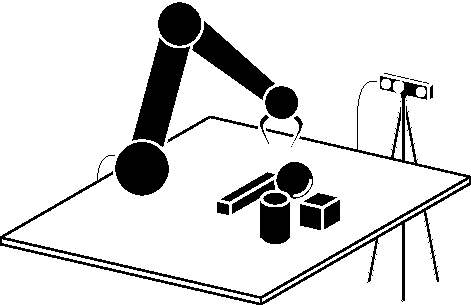
\includegraphics[height=4.3cm]{graphics/setup_sketch.pdf}
        \end{column}
        %
        \begin{column}{0.5\textwidth}%
            \centering
            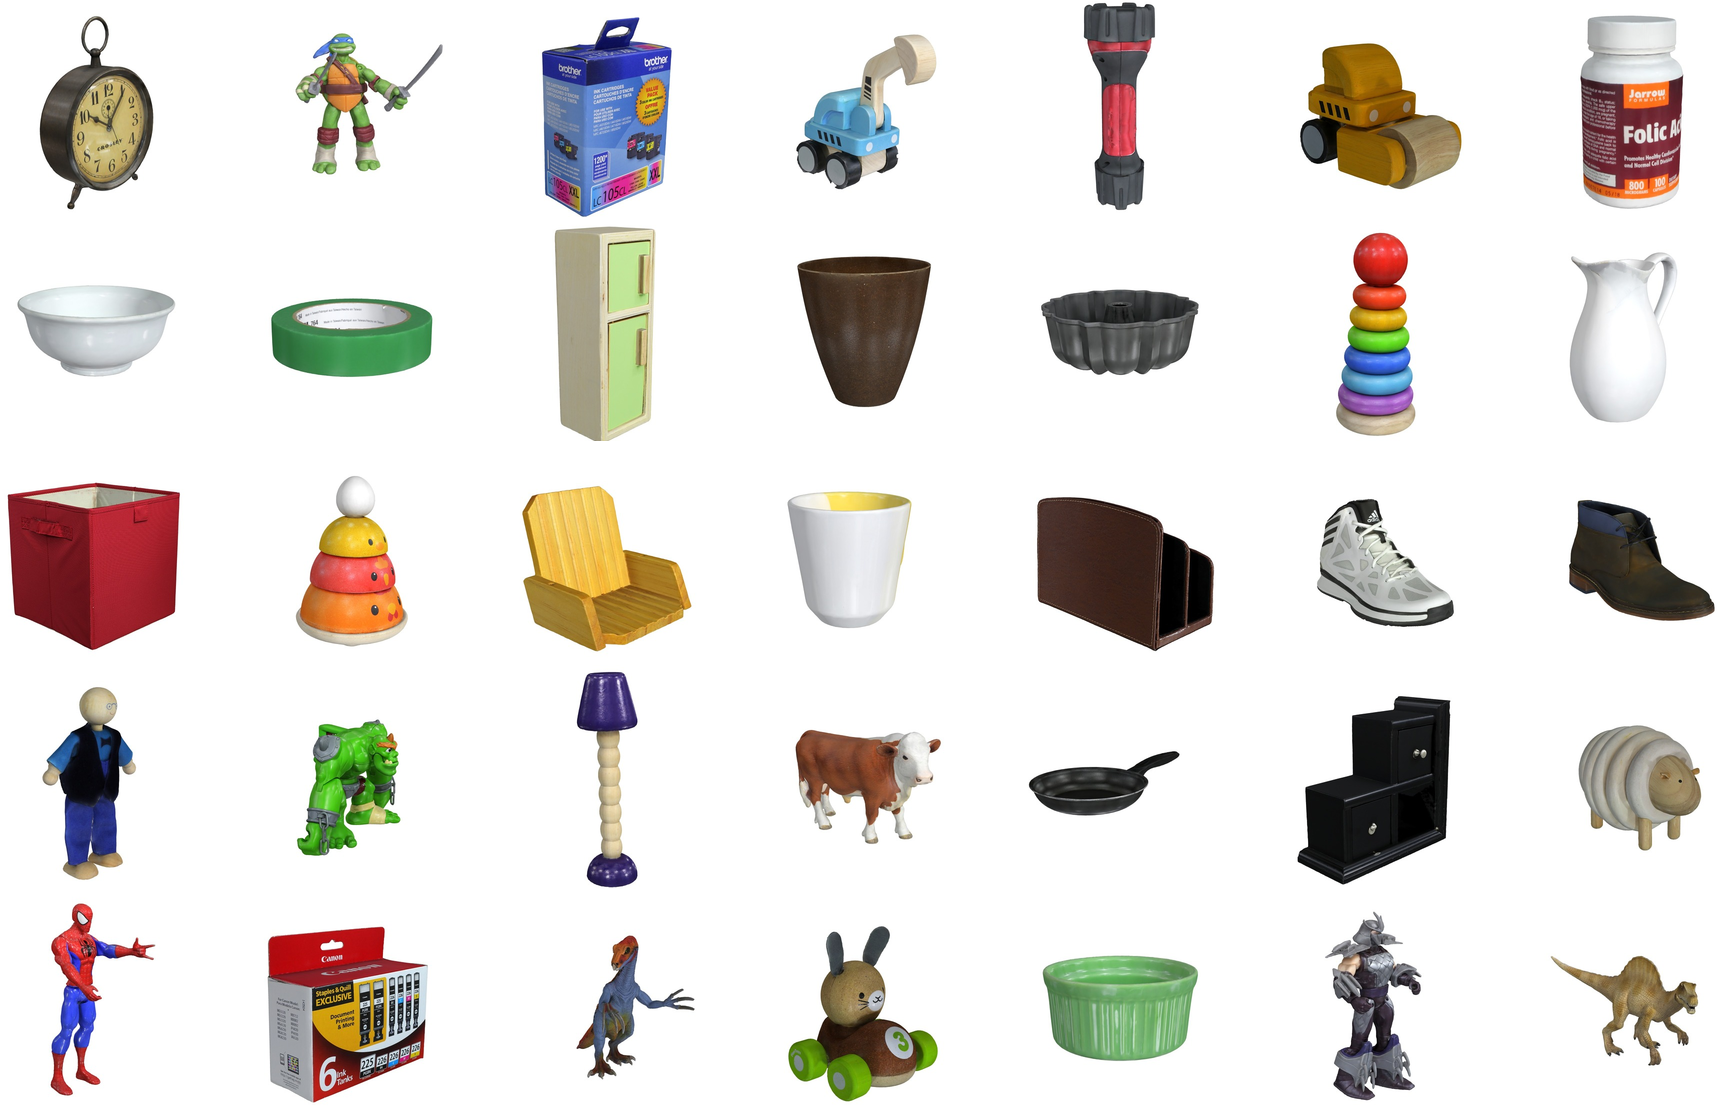
\includegraphics[height=4.3cm]{graphics/training_set.png}
        \end{column}
    \end{columns}
\end{frame}

\begin{frame}{Vision-Based Robotic Grasping of Diverse Objects}{Approach}
    \begin{columns}%
        \begin{column}{0.375\textwidth}%
            \begin{block}{Approaches}
                \begin{itemize}
                    \item Analytical
                    \item Empirical
                          \begin{itemize}
                              \item Supervised learning
                              \item Imitation learning
                              \item \only<1>{Reinforcement learning}\only<2>{\textbf{Reinforcement learning}}
                          \end{itemize}
                \end{itemize}
            \end{block}
        \end{column}
        %
        \begin{column}{0.625\textwidth}%
            \centering
            \onslide<2>{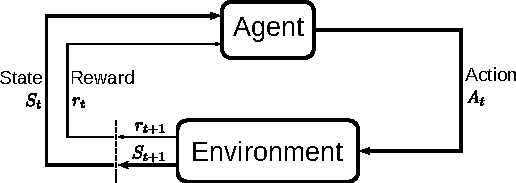
\includegraphics[width=\textwidth]{graphics/mdp_loop.pdf}}
        \end{column}
    \end{columns}
\end{frame}


\section{Task Definition}

\begin{frame}{Task Definition}{}
    \begin{columns}%
        \begin{column}{0.28\textwidth}%
            \begin{block}{Agent}
                \begin{itemize}
                    \item High-level controller
                          \begin{itemize}
                              \item Gripper pose
                              \item Gripper action
                          \end{itemize}
                \end{itemize}
            \end{block}
        \end{column}
        %
        \begin{column}{0.32\textwidth}%
            \begin{block}{Environment}
                \begin{itemize}
                    \item Objects
                    \item Robot
                          \begin{itemize}
                              \item Low-level controllers
                          \end{itemize}
                    \item Physics and visuals
                \end{itemize}
            \end{block}
        \end{column}
        %
        \begin{column}{0.35\textwidth}%
            \begin{block}{Episodic Task}
                \begin{itemize}
                    \item Success
                          \begin{itemize}
                              \item Lifting an object
                          \end{itemize}
                    \item Failure
                          \begin{itemize}
                              \item Pushing all objects away
                          \end{itemize}
                    \item Max 100 time steps
                          \begin{itemize}
                              \item \textasciitilde 40 s (simulation)
                          \end{itemize}
                \end{itemize}
            \end{block}
        \end{column}
    \end{columns}
\end{frame}

\begin{frame}{Task Definition}{Action Space}
    \begin{columns}%
        \begin{column}{0.4\textwidth}%
            \begin{block}{Actions in Cartesian Space}
                \begin{itemize}
                    \item Translational displacement
                          \begin{itemize}
                              \item \(d_{x}\)
                              \item \(d_{y}\)
                              \item \(d_{z}\)
                          \end{itemize}
                    \item Gripper rotation
                          \begin{itemize}
                              \item \(d_{\phi}\)
                          \end{itemize}
                    \item Gripper actions (open/close)
                          \begin{itemize}
                              \item \(g\)
                          \end{itemize}
                \end{itemize}
            \end{block}
        \end{column}
        %
        \begin{column}{0.6\textwidth}%
            \centering
            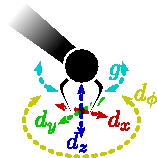
\includegraphics[height=6cm]{graphics/action_space.pdf}
        \end{column}
    \end{columns}
\end{frame}

\begin{frame}{Task Definition}{Observation Space}
    \begin{columns}%
        \begin{column}{0.6\textwidth}%
            \centering
            \only<1>{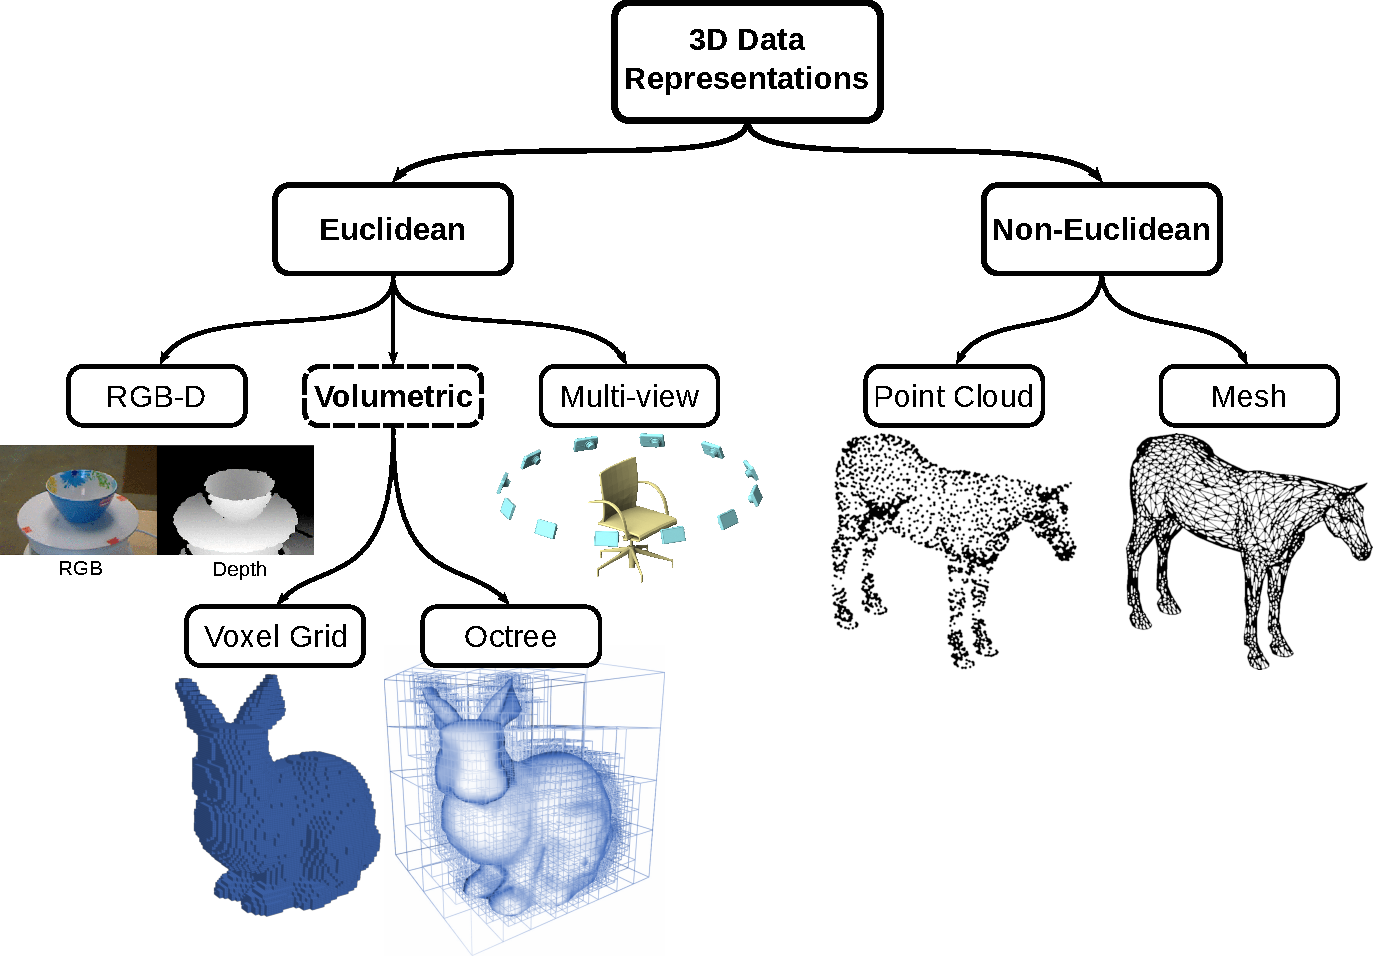
\includegraphics[height=5.85cm]{graphics/3d_data_representations.pdf}}\only<2->{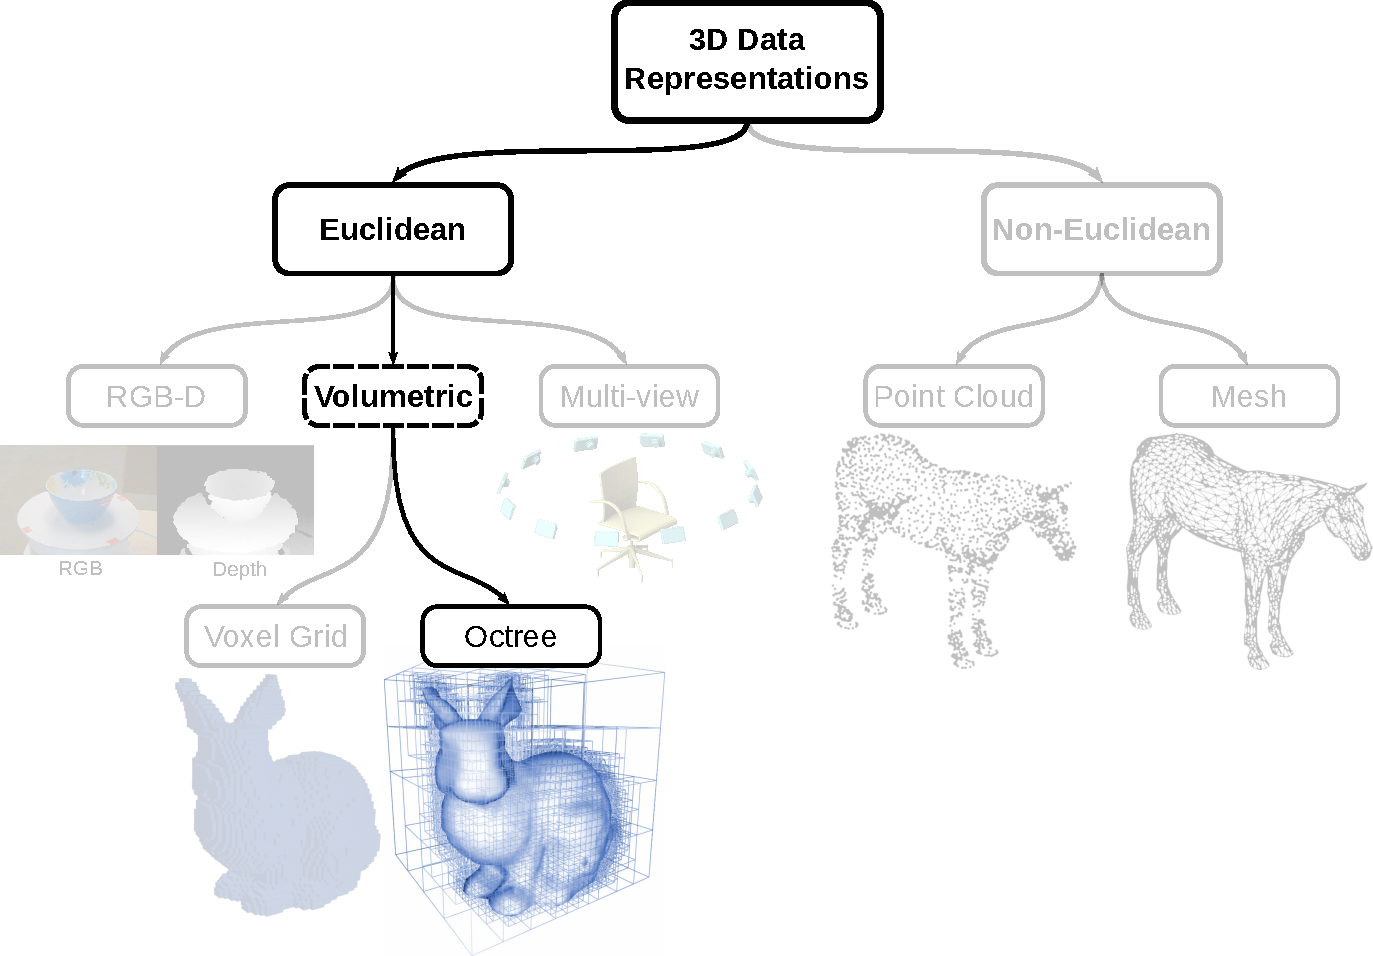
\includegraphics[height=5.85cm]{graphics/3d_data_representations_only_octree.pdf}}
        \end{column}
        %
        \begin{column}{0.4\textwidth}%
            \onslide<3>{
                \begin{block}{Proprioceptive Observations}
                    \begin{itemize}
                        \item Gripper position
                        \item Gripper rotation
                        \item Gripper state
                    \end{itemize}
                \end{block}
            }
        \end{column}
    \end{columns}
    \only<1>{\footnoteref{}}\only<2->{\footnoteref{Wang et al. 2017. O-CNN: Octree-based Convolutional Neural Networks for 3D Shape Analysis. ACM Trans. Graph. (SIGGRAPH) 36, 4, Article 72.}}
\end{frame}

\begin{frame}{Task Definition}{Observation Space - Construction of Octree}
    \centering
    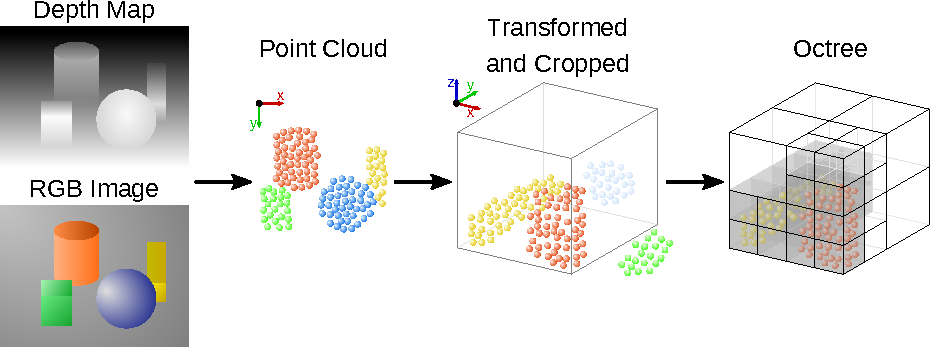
\includegraphics[width=\textwidth]{graphics/octree_creation_sketch.pdf}
\end{frame}

\begin{frame}{Task Definition}{Observation Space - Features and Stacks}
    \begin{columns}%
        \begin{column}{0.5\textwidth}%
            \begin{block}{Features}
                \begin{itemize}
                    \item Spatial
                          \begin{itemize}
                              \item Average normal vector \(\overline{n}\)
                              \item Average distance to points \(\overline{d}\)
                          \end{itemize}
                    \item Colour
                          \begin{itemize}
                              \item Average intensity of RGB channels \(\overline{rgb}\)
                          \end{itemize}
                \end{itemize}
            \end{block}
            \begin{block}{Observation Stacking}
                \begin{itemize}
                    \item Three consecutive observations
                \end{itemize}
            \end{block}
        \end{column}
        %
        \begin{column}{0.5\textwidth}%
            \centering
            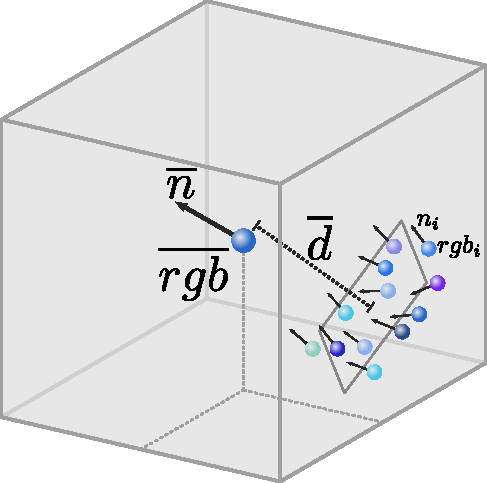
\includegraphics[height=5cm]{graphics/octree_features_sketch.pdf}
        \end{column}
    \end{columns}
\end{frame}

\begin{frame}{Task Definition}{Reward Function}
    \begin{columns}%
        \begin{column}{0.5\textwidth}%
            \begin{block}{Composite Reward}
                \begin{itemize}
                    \item Reach
                          \begin{itemize}
                              \item \(+1\) (\(7^{0}\))
                          \end{itemize}
                    \item Touch
                          \begin{itemize}
                              \item \(+7\) (\(7^{1}\))
                          \end{itemize}
                    \item Grasp
                          \begin{itemize}
                              \item \(+49\) (\(7^{2}\))
                          \end{itemize}
                    \item Lift
                          \begin{itemize}
                              \item \(+343\) (\(7^{3}\))
                          \end{itemize}
                \end{itemize}
            \end{block}
        \end{column}
        %
        \begin{column}{0.5\textwidth}%
            \begin{block}{Recurring Reward}
                \begin{itemize}
                    \item Collision with ground/table
                          \begin{itemize}
                              \item \(-1\)
                          \end{itemize}
                    \item Incentive to act quickly
                          \begin{itemize}
                              \item \(-0.005\)
                          \end{itemize}
                \end{itemize}
            \end{block}
        \end{column}
    \end{columns}
\end{frame}

\begin{frame}{Task Definition}{Summary}
    \begin{columns}%
        \begin{column}{0.3\textwidth}%
            \centering
            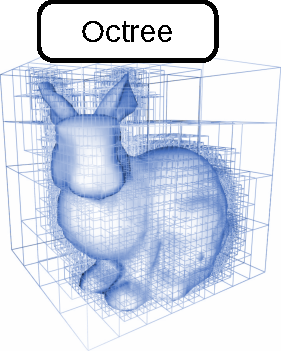
\includegraphics[height=5cm]{graphics/3d_data_representations_only_octree_cropped.pdf}
        \end{column}
        %
        \begin{column}{0.3\textwidth}%
            \centering
            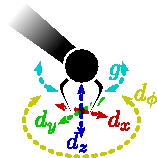
\includegraphics[height=4cm]{graphics/action_space.pdf}
        \end{column}
        %
        \begin{column}{0.35\textwidth}%
            \begin{block}{Reward Function}
                \begin{itemize}
                    \item Composite
                          \begin{itemize}
                              \item Reach
                              \item Touch
                              \item Grasp
                              \item Lift
                          \end{itemize}
                    \item Collision with ground/table
                    \item Incentive to act quickly
                \end{itemize}
            \end{block}
        \end{column}
    \end{columns}
\end{frame}


\section{Deep Reinforcement Learning Algorithms and Network Architecture}

\begin{frame}{Deep Reinforcement Learning}{Algorithms}
    \begin{columns}%
        \begin{column}{0.3\textwidth}%
            \begin{block}{Actor-Critic Algorithms}
                \begin{itemize}
                    \item TD3
                    \item SAC
                    \item TQC
                \end{itemize}
            \end{block}
            \begin{block}{Implementation}
                \begin{itemize}
                    \item Stable Baselines3
                \end{itemize}
            \end{block}
        \end{column}
        %
        \begin{column}{0.7\textwidth}%
            \centering
            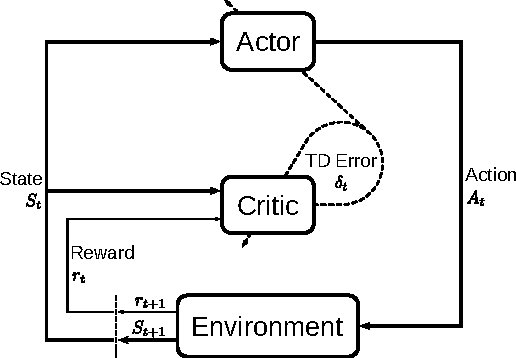
\includegraphics[height=6cm]{graphics/actor_critic_loop.pdf}
        \end{column}
    \end{columns}
\end{frame}

\begin{frame}{Deep Reinforcement Learning}{Octree-Based Feature Extractor}
    \centering
    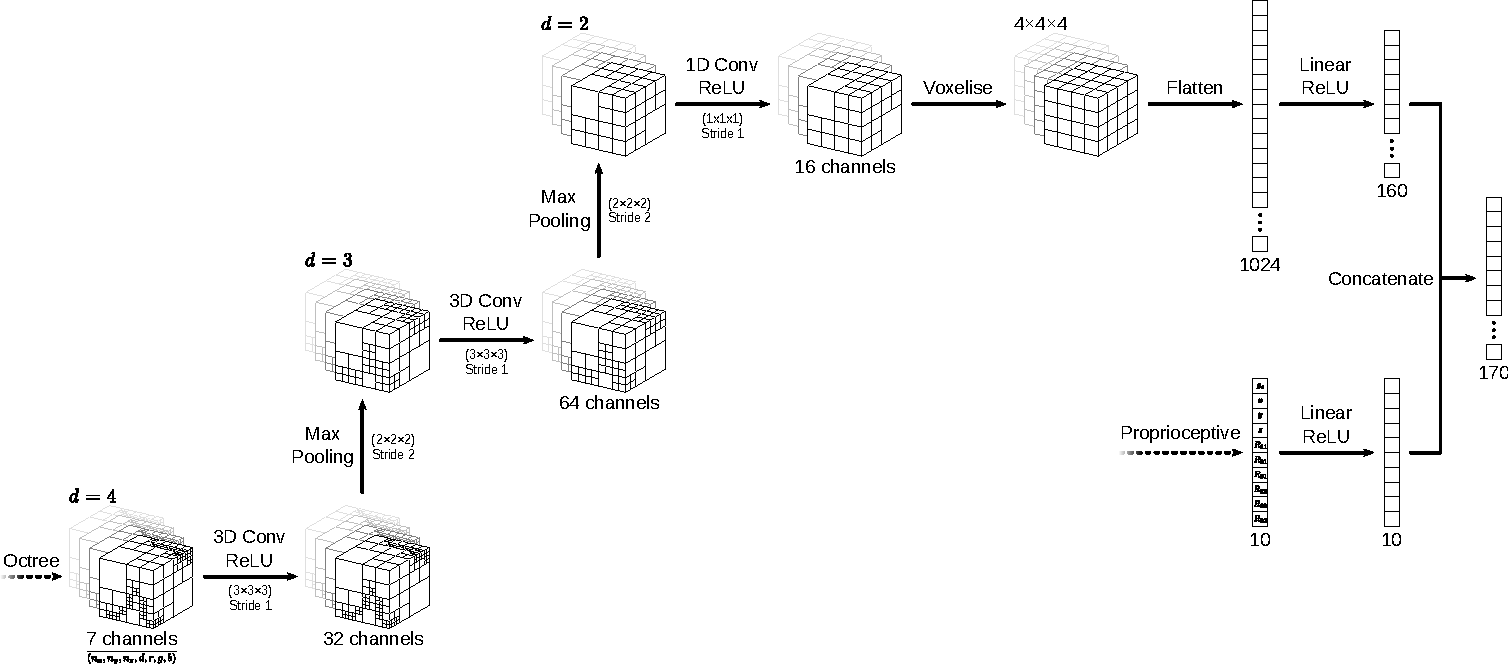
\includegraphics[width=\textwidth]{graphics/feature_extractor.pdf}
\end{frame}

\begin{frame}{Deep Reinforcement Learning}{Full Actor-Critic Network Architecture}
    \centering
    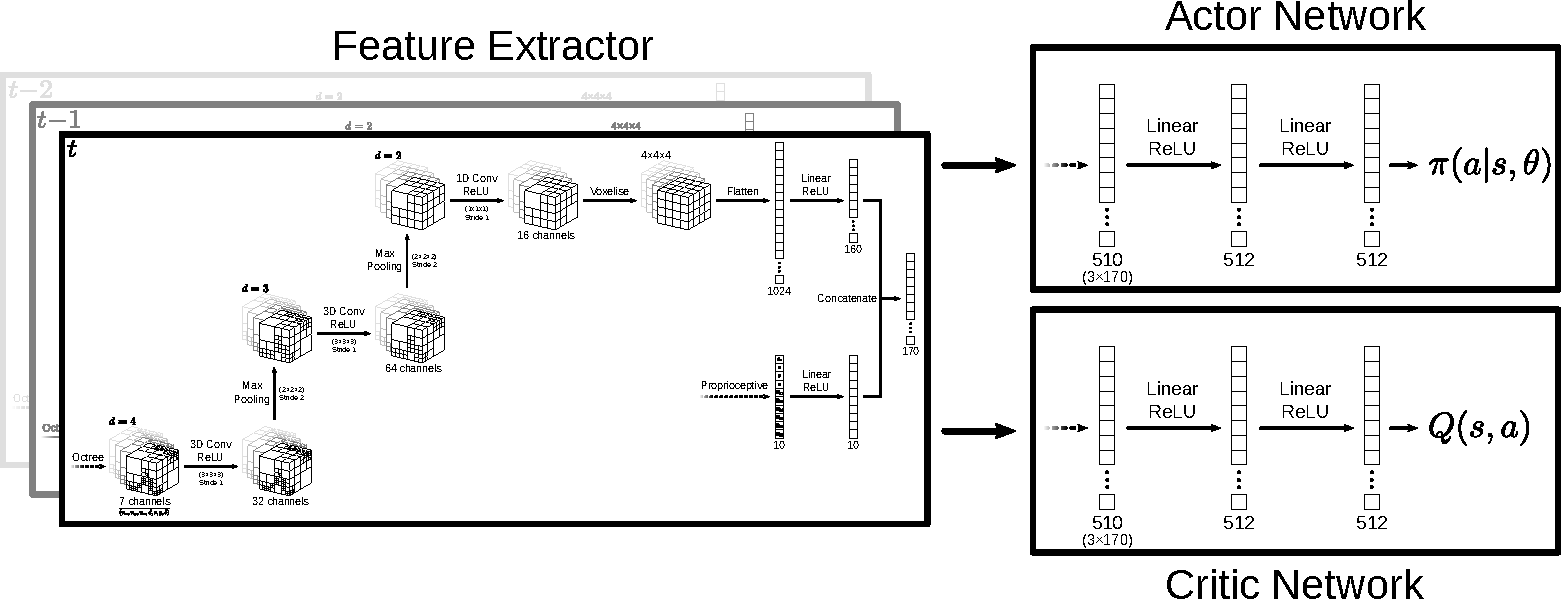
\includegraphics[width=\textwidth]{graphics/actor_critic_network_full.pdf}
\end{frame}


\section{Simulation Environment}

\begin{frame}{Simulation Environment}{Selection}
    \begin{columns}%
        \begin{column}{0.35\textwidth}%
            \begin{block}{Simulators}
                \begin{itemize}
                    \item MuJoCo
                    \item PyBullet
                    \item Gazebo Classic
                    \item \only<1>{Ignition Gazebo}\only<2>{\textbf{Ignition Gazebo}}
                    \item Isaac
                    \item Webots
                    \item Unreal Engine
                    \item Unity
                    \item Unigine
                    \item RaiSim
                    \item ...
                \end{itemize}
            \end{block}
        \end{column}
        %
        \begin{column}{0.65\textwidth}%
            \centering
            \onslide<2>{
\includegraphics[width=0.65\textwidth]{graphics/ignition_logo.pdf}}
        \end{column}
    \end{columns}
\end{frame}

\begin{frame}{Simulation Environment}{Ignition Gazebo}
    \begin{columns}%
        \begin{column}{0.4\textwidth}%
            \begin{block}{Physics}
                \vspace{0.2cm}

                \centering
                
\includegraphics[width=0.7\textwidth]{graphics/dart_logo.png}
            \end{block}

            \vspace{1cm}

            \begin{block}{Rendering}
                \vspace{0.2cm}

                \centering
                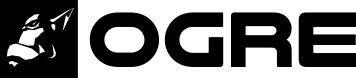
\includegraphics[width=0.7\textwidth]{graphics/ogre_logo.png}
            \end{block}
        \end{column}
        %
        \begin{column}{0.6\textwidth}%
            \onslide<2>{
                \begin{block}{Gym-Ignition}
                    \begin{itemize}
                        \item Interface for Ignition Gazebo
                        \item Tooling for creation of OpenAI Gym environments%
                              \begin{itemize}
                                  \item Compatibility with RL frameworks
                              \end{itemize}
                    \end{itemize}
                \end{block}
            }
        \end{column}
    \end{columns}
    \only<1>{\footnoteref{}}\only<2->{\footnoteref{Ferigo et al. 2020. Gym-Ignition: Reproducible Robotic Simulations for Reinforcement Learning. In 2020 IEEE/SICE International Symposium on System Integration (SII). 885–890.}}
\end{frame}

\begin{frame}{Simulation Environment}{Datasets}
    \centering
    \includegraphics[height=6.5cm]{graphics/datasets_full.png}
\end{frame}

\begin{frame}{Simulation Environment}{Domain Randomisation}
    \centering
    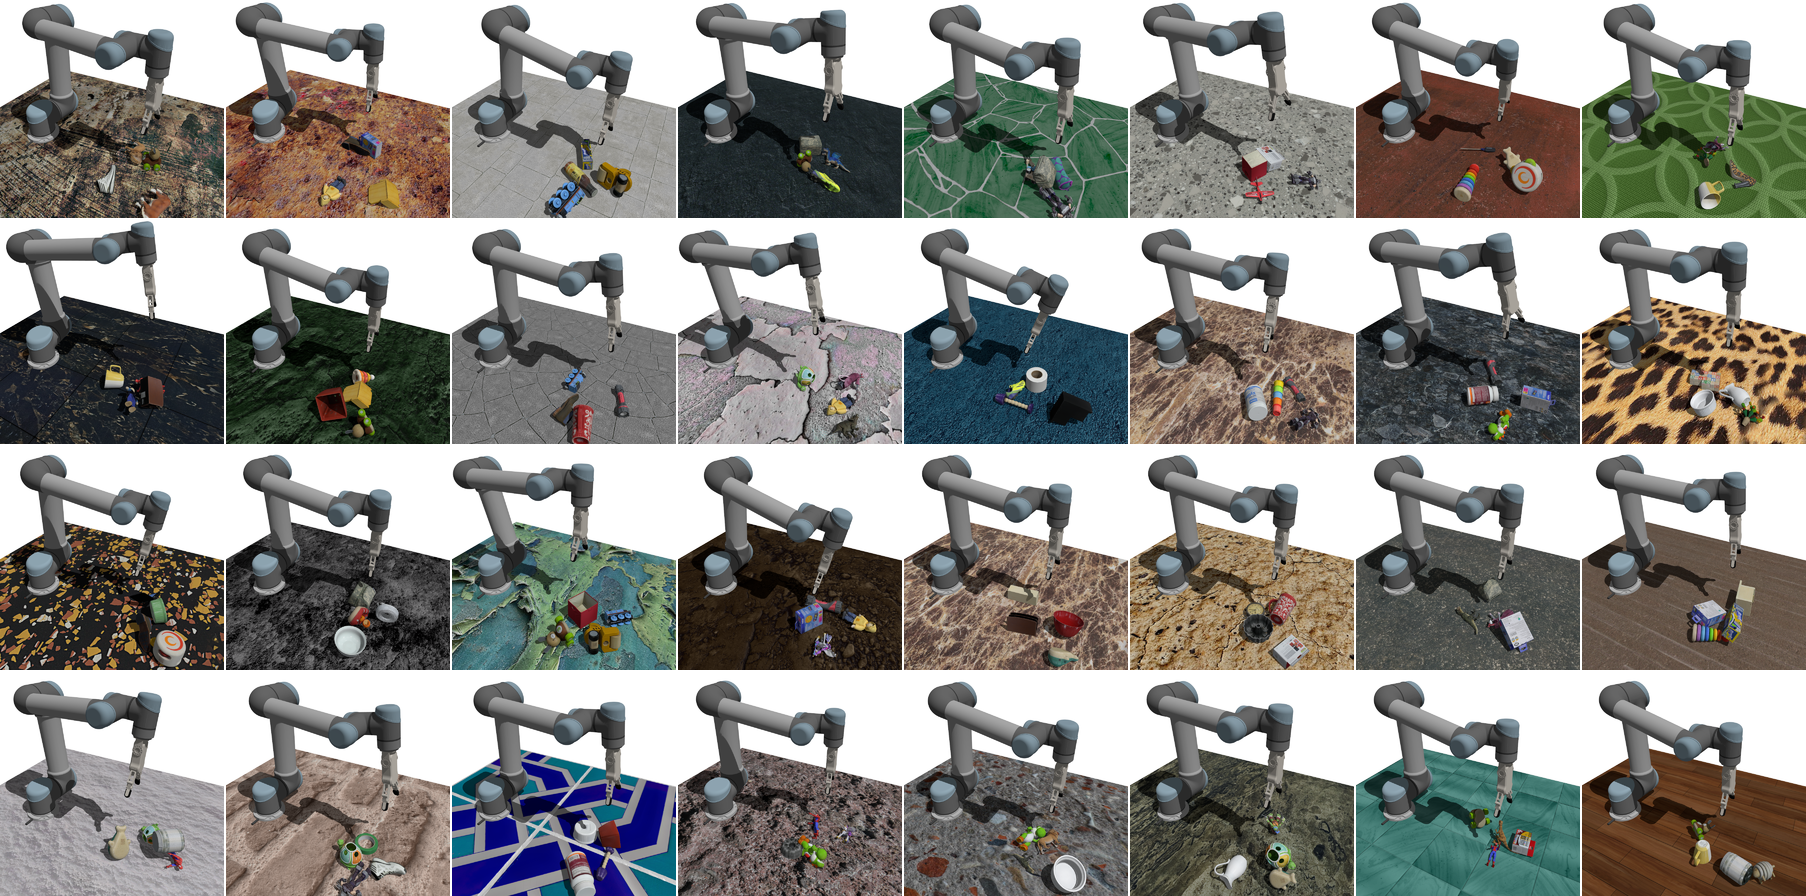
\includegraphics[height=6.5cm]{graphics/domain_randomisation.png}
\end{frame}

\begin{frame}{Simulation Environment}{Domain Randomisation}
    \begin{columns}%
        \begin{column}{0.35\textwidth}%
            \begin{block}{Random}
                \begin{itemize}
                    \item Object
                          \begin{itemize}
                              \item Model
                              \item Scale
                              \item Mass
                              \item Friction
                              \item Pose
                          \end{itemize}
                    \item Ground plane texture
                    \item Initial robot configuration
                    \item Camera
                          \begin{itemize}
                              \item Pose
                              \item Sensory noise
                          \end{itemize}
                \end{itemize}
            \end{block}
        \end{column}
        %
        \begin{column}{0.65\textwidth}%
            \centering
            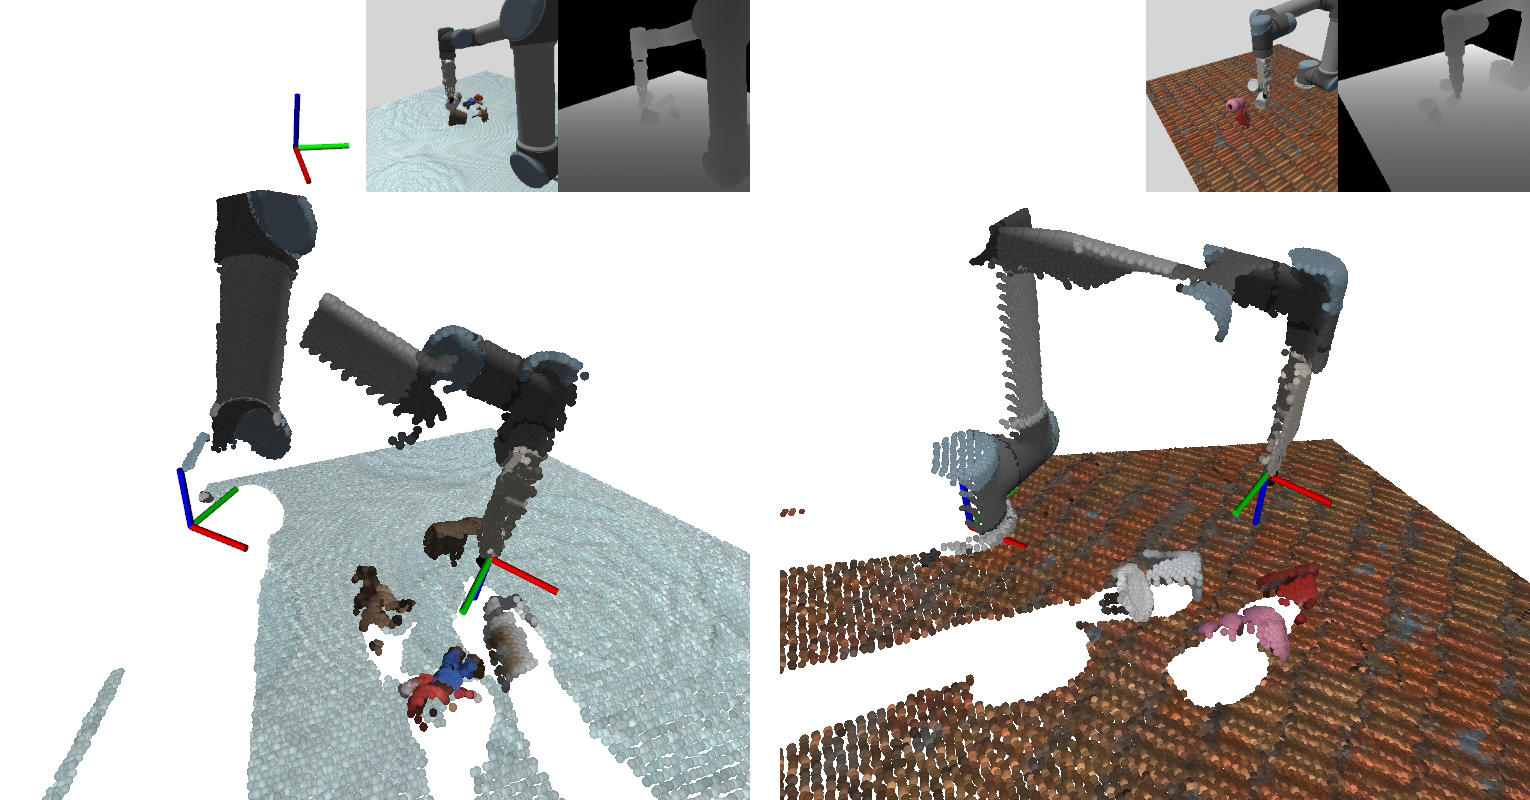
\includegraphics[height=4.75cm]{graphics/random_camera_pose.png}
        \end{column}
    \end{columns}
\end{frame}

\begin{frame}{Simulation Environment}{Environment for Training}
    \centering
    \only<1>{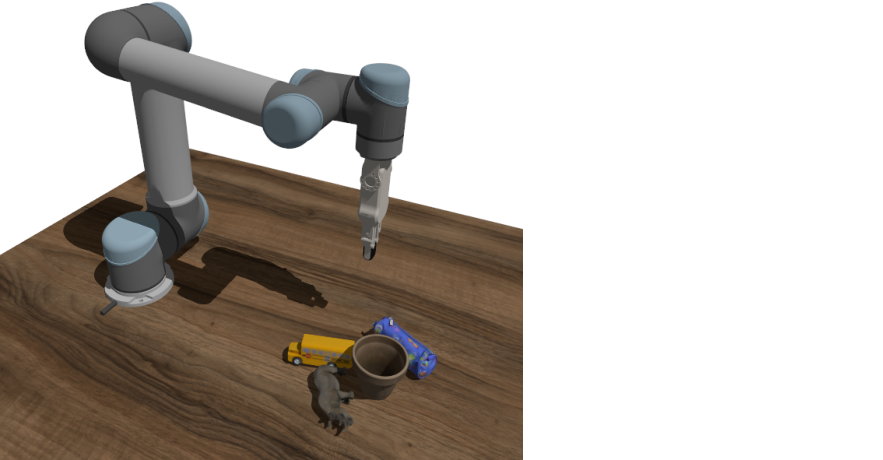
\includegraphics[height=6cm]{graphics/octree_example_1.pdf}}\only<2>{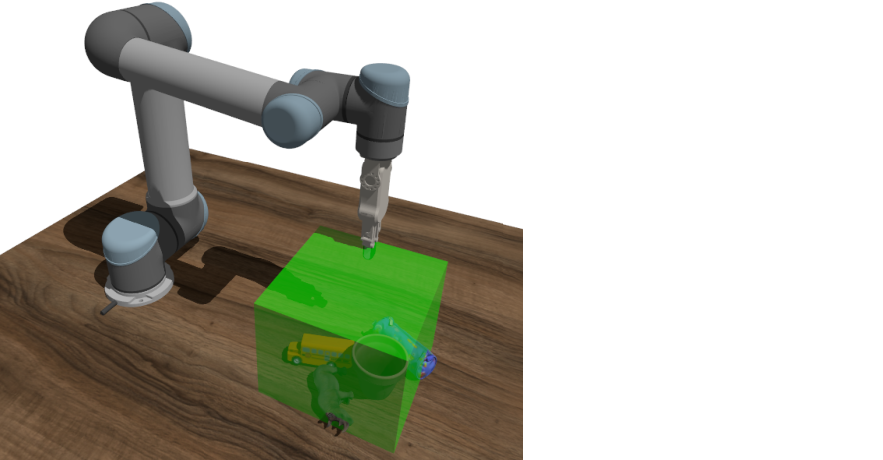
\includegraphics[height=6cm]{graphics/octree_example_2.pdf}}\only<3>{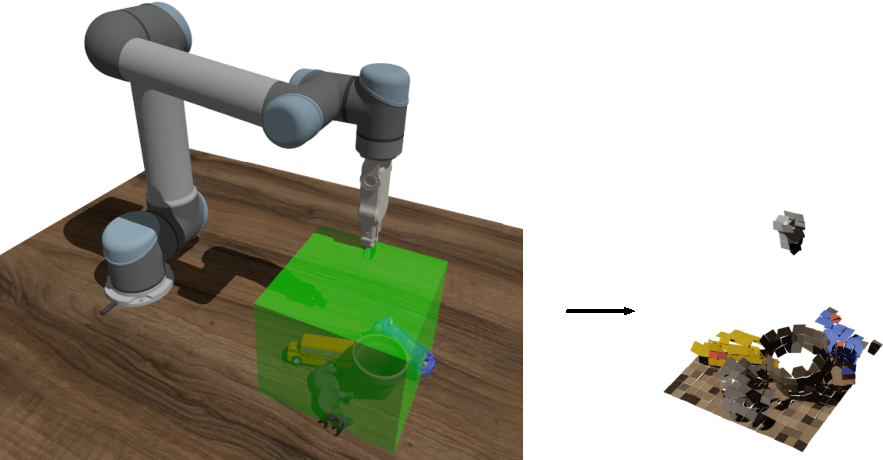
\includegraphics[height=6cm]{graphics/octree_example_3.pdf}}
\end{frame}


\section{Training}

\begin{frame}{Training}{Hyperparameters}
    \begin{columns}%
        \begin{column}{0.3\textwidth}%
            \begin{block}{Optimisation}
                \begin{itemize}
                    \item Automatic (Optuna)
                    \item Manual
                \end{itemize}
            \end{block}
        \end{column}
        %
        \begin{column}{0.7\textwidth}%
            \centering
            \resizebox{0.85\textwidth}{!}{%
                \begin{tabular}{l|ccc}
                    \textbf{Hyperparameter}     & \textbf{TD3}                                                    & \textbf{SAC}                                 & \textbf{TQC} \\ \hline
                    Optimisation Algorithm      & \multicolumn{3}{c}{\begin{tabular}[c]{@{}c@{}}Adam\end{tabular}}                                                                            \\
                    Learning Rate Schedule      & \multicolumn{3}{c}{Linear, \(1.5 \cdot 10^{-4} \rightarrow 0\)}                                                               \\
                    Mini-batch Size             & \multicolumn{3}{c}{\(32\)}                                                                                                    \\
                    Update Frequency            & \multicolumn{3}{c}{After Every Episode}                                                                                       \\
                    Gradient Steps per Update   & \multicolumn{3}{c}{\(100\)}                                                                                                   \\
                    Replay Buffer Size          & \multicolumn{3}{c}{\(40000\)}                                                                                                 \\
                    Discount Factor \(\gamma\)  & \multicolumn{3}{c}{\(0.999\)}                                                                                                 \\
                    Target Update Rate \(\tau\) & \multicolumn{3}{c}{\(5 \cdot 10^{-5}\)}                                                                                       \\
                    Number of Critics           & \multicolumn{3}{c}{\(2\)}                                                                                                     \\
                    Activation Function         & \multicolumn{3}{c}{ReLU}                                                                                                      \\
                    Exploratory Action Noise    & \multicolumn{3}{c}{\(\mathcal{N}(0, 0.025)\)}                                                                                 \\ \hline
                    Target Policy Noise         & \(\mathcal{N}(0, 0.25)\)                                        & ---                                          & ---          \\ \hline
                    Initial Entropy Coefficient & ---                                                             & \multicolumn{2}{c}{\(0.1\)}                                 \\
                    Entropy Target              & ---                                                             & \multicolumn{2}{c}{\(-dim(\mathcal{A})=-5\)}                \\ \hline
                    Number of Atoms             & ---                                                             & ---                                          & \(25\)       \\
                    Number of Truncated Atoms   & ---                                                             & ---                                          & \(3\)        \\
                \end{tabular}
            }
        \end{column}
    \end{columns}
\end{frame}

\begin{frame}{Training}{Demonstrations and Curriculum}
    \begin{columns}%
        \begin{column}{0.5\textwidth}%
            \begin{block}{Demonstrations}
                \begin{itemize}
                    \item Automatic collection of samples
                          \begin{itemize}
                              \item Simple scripted policy
                                    \begin{itemize}
                                        \item 19\% success rate
                                    \end{itemize}
                          \end{itemize}
                    \item 5k Collected transitions
                          \begin{itemize}
                              \item Replaced after 40k steps (buffer size)
                          \end{itemize}
                \end{itemize}
            \end{block}
        \end{column}
        %
        \begin{column}{0.5\textwidth}%
            \begin{block}{Curriculum}
                \begin{itemize}
                    \item Scaling of environment difficulty
                          \begin{itemize}
                              \item Number of objects
                                    \begin{itemize}
                                        \item 1 \(\rightarrow\) 4
                                    \end{itemize}
                              \item Spawn area
                                    \begin{itemize}
                                        \item 2.4 cm~\(\times\)~2.4 cm \(\rightarrow\) 24 cm~\(\times\)~24 cm
                                    \end{itemize}
                          \end{itemize}
                    \item Full problem at 60\% success rate
                \end{itemize}
            \end{block}
        \end{column}
    \end{columns}
\end{frame}

\section{Results}

\begin{frame}{Results}{Overview}
    \begin{columns}%
        \begin{column}{0.5\textwidth}%
            \begin{block}{Experiments}
                \begin{itemize}
                    \item Comparison of actor-critic algorithms
                    \item Comparison of 2D/2.5D/3D observations
                    \item Invariance to robot
                    \item Sim-to-real transfer
                \end{itemize}
            \end{block}
        \end{column}
        %
        \begin{column}{0.5\textwidth}%
            \begin{block}{Ablation Studies}
                \begin{itemize}
                    \item No demonstrations
                    \item No curriculum
                    \item No colour features
                    \item No proprioceptive
                    \item Shared/separate feature extractor
                          \begin{itemize}
                              \item Among actor and critics
                              \item Among observation stacks
                          \end{itemize}
                \end{itemize}
            \end{block}
        \end{column}
    \end{columns}
\end{frame}

\begin{frame}{Results}{Comparison of Actor-Critic Algorithms}
    \begin{columns}%
        \begin{column}{0.55\textwidth}%
            \centering
            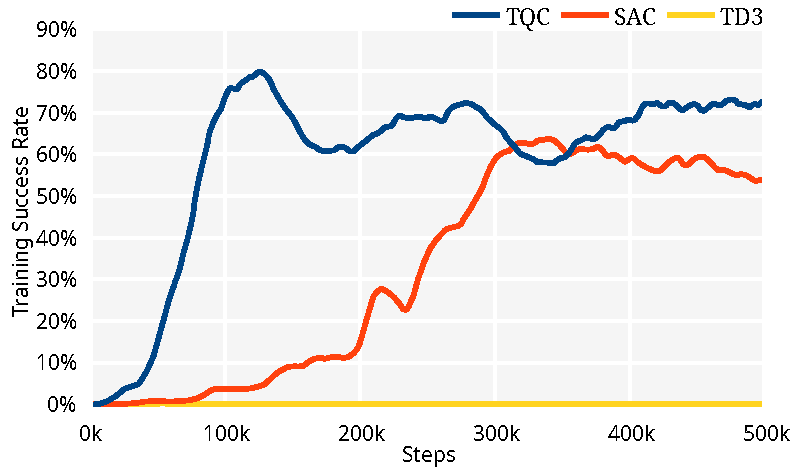
\includegraphics[height=4.25cm]{graphics/results_actor_critic.pdf}
        \end{column}
        %
        \begin{column}{0.45\textwidth}%
            \centering
            \begin{tabular}{c|ccc}
                                               & \textbf{TQC} & \textbf{SAC} & \textbf{TD3} \\ \hline
                \begin{tabular}[c|]{@{}c@{}}Success\\Rate\end{tabular} & 77\%         & 64\%         & 0\%          \\[4mm]
                \begin{tabular}[c|]{@{}c@{}}Episode\\Length\end{tabular} & 14.0         & 29.8         & ---
            \end{tabular}
        \end{column}
    \end{columns}
\end{frame}

\begin{frame}{Results}{Agent Trained with TQC (Video Example)}
    \centering
    \vspace{-0.4cm}
    \scalebox{0.25}{%
        \def \vidwidth{1500px}%
        \def \vidheight{800px}%
        \includemedia[width=\vidwidth,height=\vidheight,activate=pageopen,
            passcontext,
            transparent,
            keepaspectratio,
            final,
            noplaybutton,
            addresource=videos/sim_ur5_rg2.mp4,
            flashvars={source=videos/sim_ur5_rg2.mp4 &loop=true}
        ]{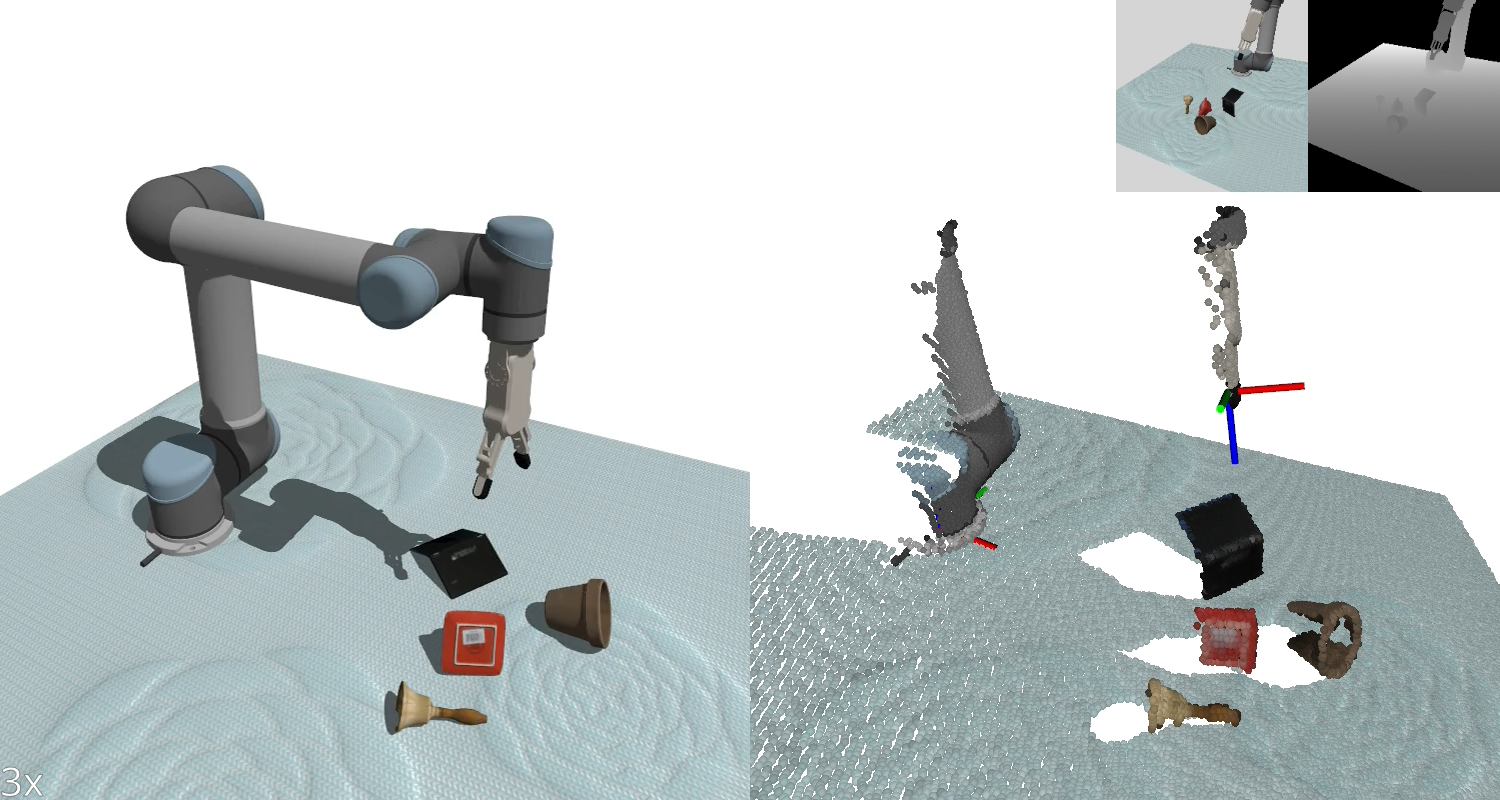
\includegraphics[width=\vidwidth,height=\vidheight]{videos/sim_ur5_rg2_0.png}}{VPlayer.swf}
    }
\end{frame}

\begin{frame}{Results}{Comparison of 2D/2.5D/3D Observations - Feature Extractor}
    \centering
    \only<1>{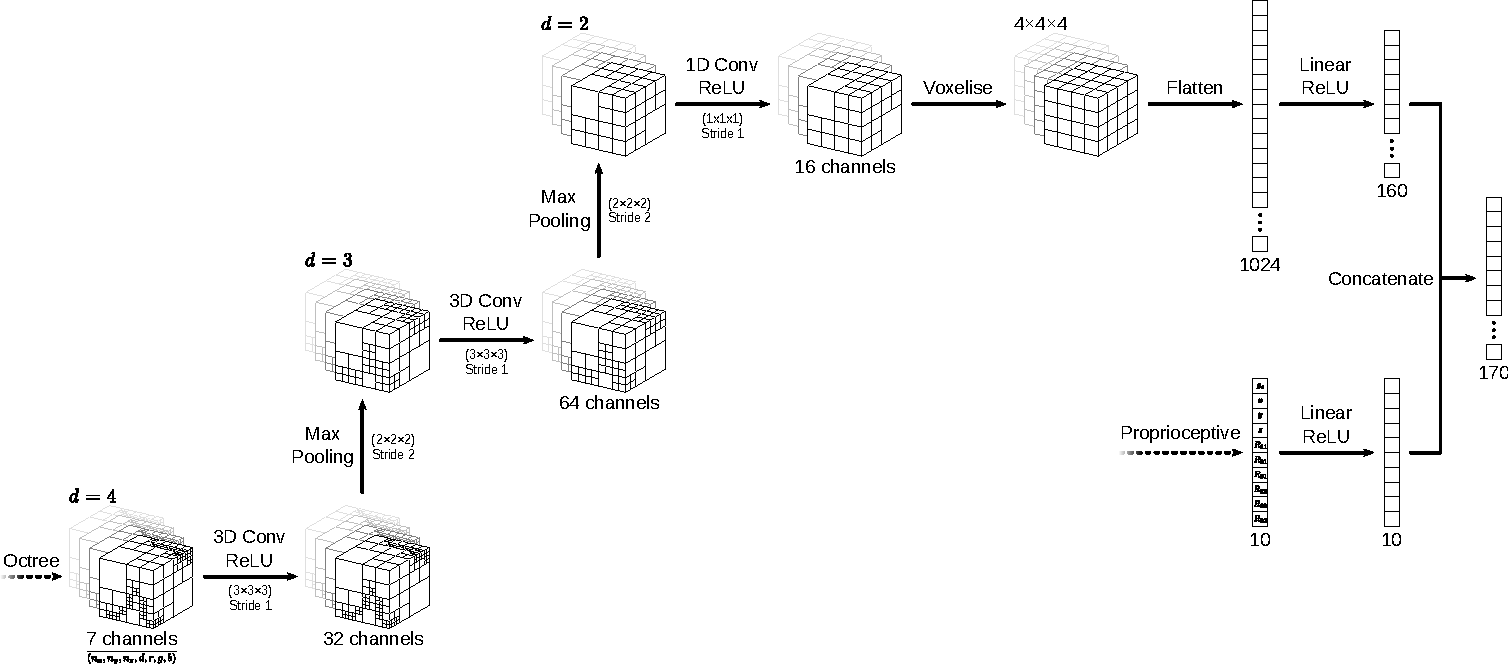
\includegraphics[width=\textwidth]{graphics/feature_extractor.pdf}}\only<2>{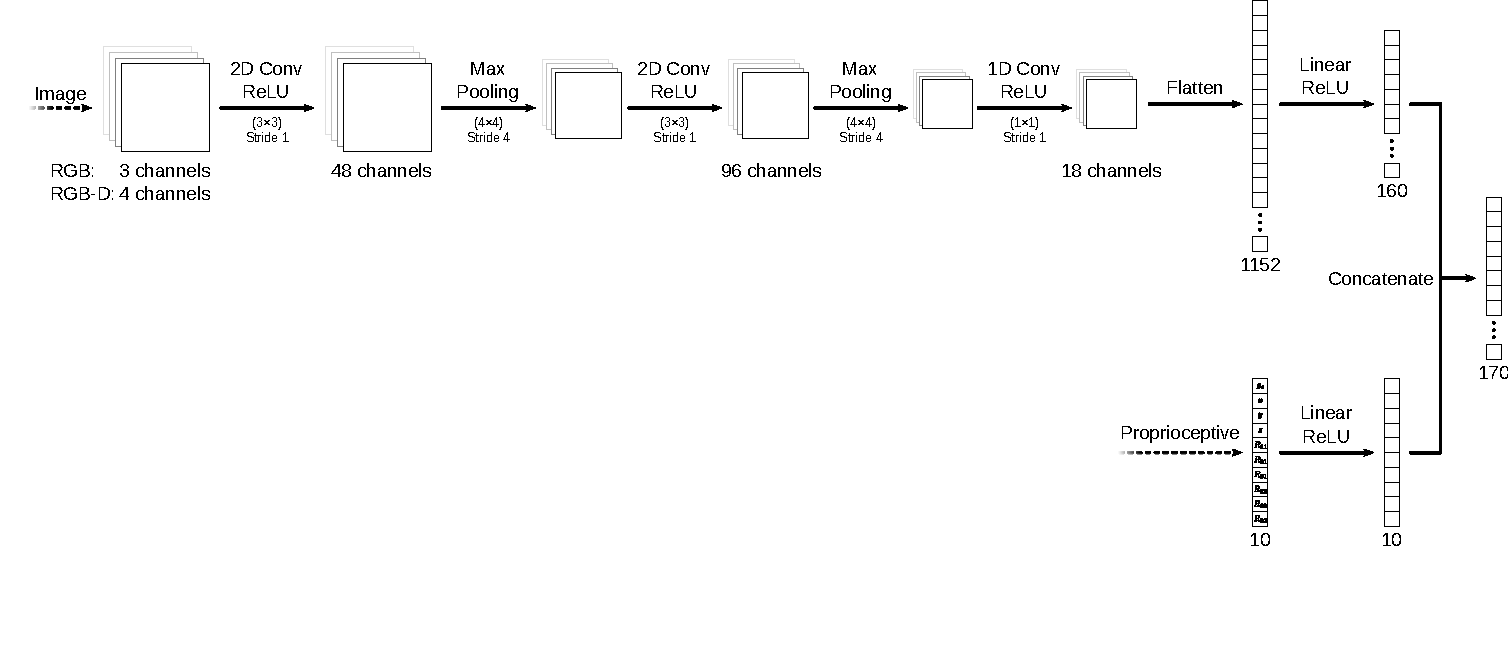
\includegraphics[width=\textwidth]{graphics/image_feature_extractor.pdf}}
\end{frame}

\begin{frame}{Results}{Comparison of 2D/2.5D/3D Observations - Random Camera Pose}
    \begin{columns}%
        \begin{column}{0.55\textwidth}%
            \centering
            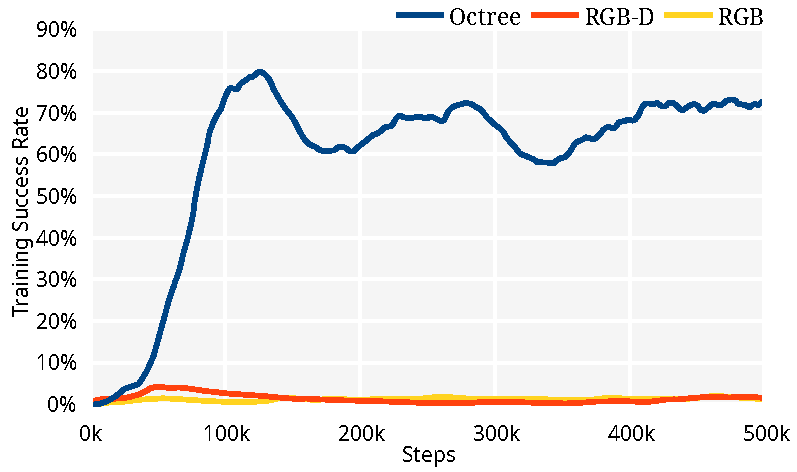
\includegraphics[height=4.25cm]{graphics/results_2d_25d_3d_random_camera_pose.pdf}
        \end{column}
        %
        \begin{column}{0.45\textwidth}%
            \centering
            \begin{tabular}{c|ccc}
                                               & \textbf{Octree} & \textbf{RGB-D} & \textbf{RGB} \\ \hline
                \begin{tabular}[c|]{@{}c@{}}Success\\Rate\end{tabular} & 77\%            & 5\%            & 3\%          \\[4mm]
                \begin{tabular}[c|]{@{}c@{}}Episode\\Length\end{tabular} & 14.0            & 36.5           & 51.0
            \end{tabular}
        \end{column}
    \end{columns}
\end{frame}

\begin{frame}{Results}{Comparison of 2D/2.5D/3D Observations - Static Camera Pose}
    \begin{columns}%
        \begin{column}{0.55\textwidth}%
            \centering
            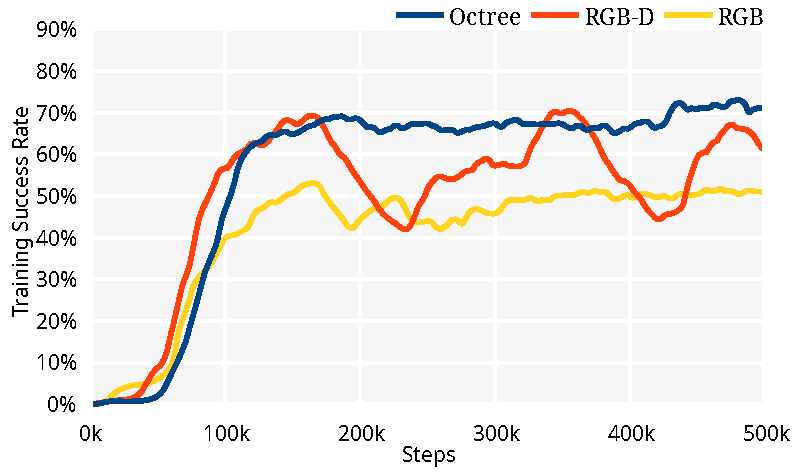
\includegraphics[height=4.25cm]{graphics/results_2d_25d_3d_static_camera_pose.pdf}
        \end{column}
        %
        \begin{column}{0.45\textwidth}%
            \centering
            \begin{tabular}{c|ccc}
                                               & \textbf{Octree} & \textbf{RGB-D} & \textbf{RGB} \\ \hline
                \begin{tabular}[c|]{@{}c@{}}Success\\Rate\end{tabular} & 81.5\%          & 59\%           & 35\%         \\[4mm]
                \begin{tabular}[c|]{@{}c@{}}Episode\\Length\end{tabular} & 24.6            & 9.4            & 9.3
            \end{tabular}
        \end{column}
    \end{columns}
\end{frame}

\begin{frame}{Results}{Invariance to Robot - Training and Evaluation}
    \begin{columns}%
        \begin{column}{0.55\textwidth}%
            \centering
            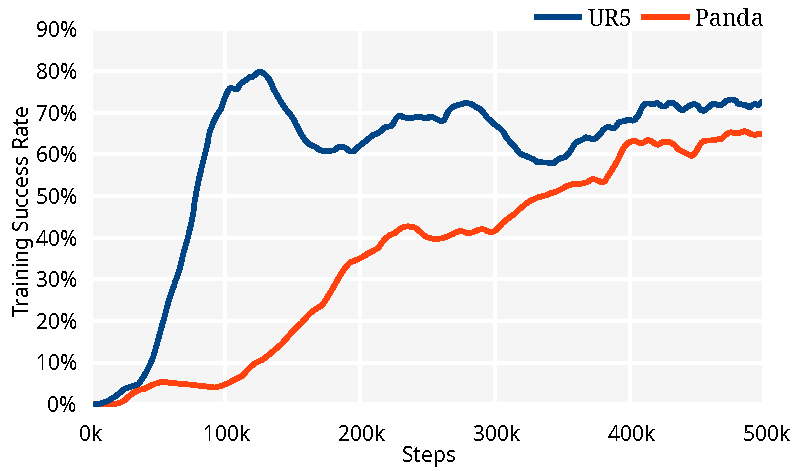
\includegraphics[height=4.25cm]{graphics/results_ue5_panda_robot.pdf}
        \end{column}
        %
        \begin{column}{0.45\textwidth}%
            \centering
            \begin{tabular}{c|cc}
                                               & \textbf{UR5} & \textbf{Panda} \\ \hline
                \begin{tabular}[c|]{@{}c@{}}Success\\Rate\end{tabular} & 77\%         & 61.5\%         \\[4mm]
                \begin{tabular}[c|]{@{}c@{}}Episode\\Length\end{tabular} & 14.0         & 27.1
            \end{tabular}
        \end{column}
    \end{columns}
\end{frame}

\begin{frame}{Results}{Invariance to Robot - Transfer of Policy}
    \centering
    \begin{columns}%
        \begin{column}{0.2875\textwidth}%
            \centering
            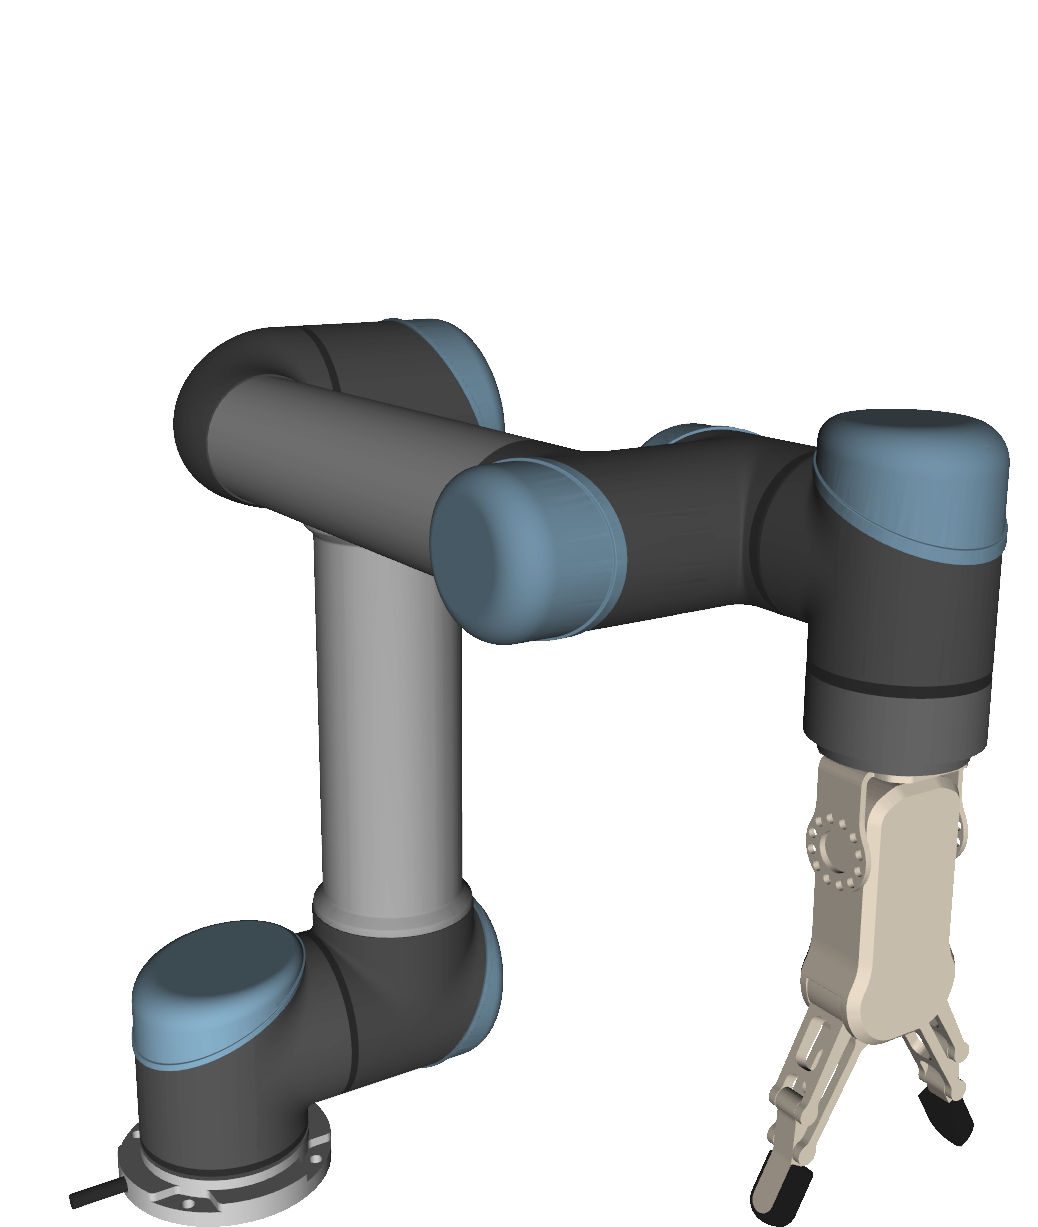
\includegraphics[height=4.3cm]{graphics/ur5_rg2.png}
        \end{column}
        %
        \begin{column}{0.425\textwidth}%
            \centering
            \begin{tabular}{cr|cc}
                                                                &                & \multicolumn{2}{c}{Evaluation}                  \\
                                                                &                & \textbf{UR5}                   & \textbf{Panda} \\ \hline
                \multirow{2}{*}{\begin{tabular}[c]{@{}c@{}}Training\end{tabular}} & \textbf{UR5}   & 77\%                           & 27.5\%         \\
                                                                & \textbf{Panda} & 75\%                           & 61.5\%
            \end{tabular}
        \end{column}
        %
        \begin{column}{0.2875\textwidth}%
            \centering
            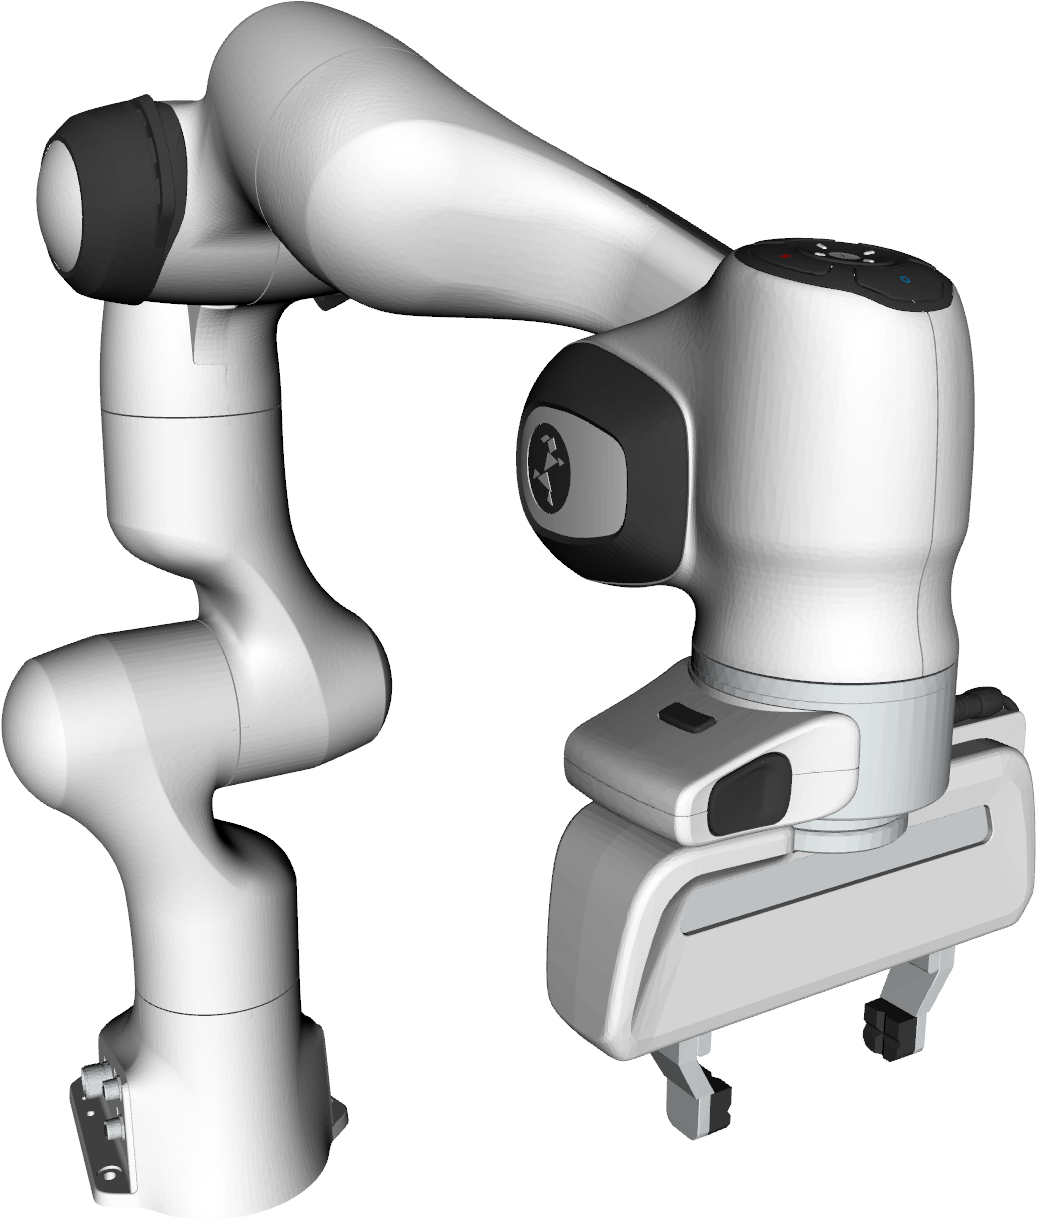
\includegraphics[height=4.3cm]{graphics/panda.png}
        \end{column}
    \end{columns}
\end{frame}

\begin{frame}{Results}{Policy Trained on Panda (Video Example)}
    \centering
    \vspace{-0.4cm}
    \scalebox{0.25}{%
        \def \vidwidth{1500px}%
        \def \vidheight{800px}%
        \includemedia[width=\vidwidth,height=\vidheight,activate=pageopen,
            passcontext,
            transparent,
            keepaspectratio,
            final,
            noplaybutton,
            addresource=videos/sim_panda.mp4,
            flashvars={source=videos/sim_panda.mp4 &loop=true}
        ]{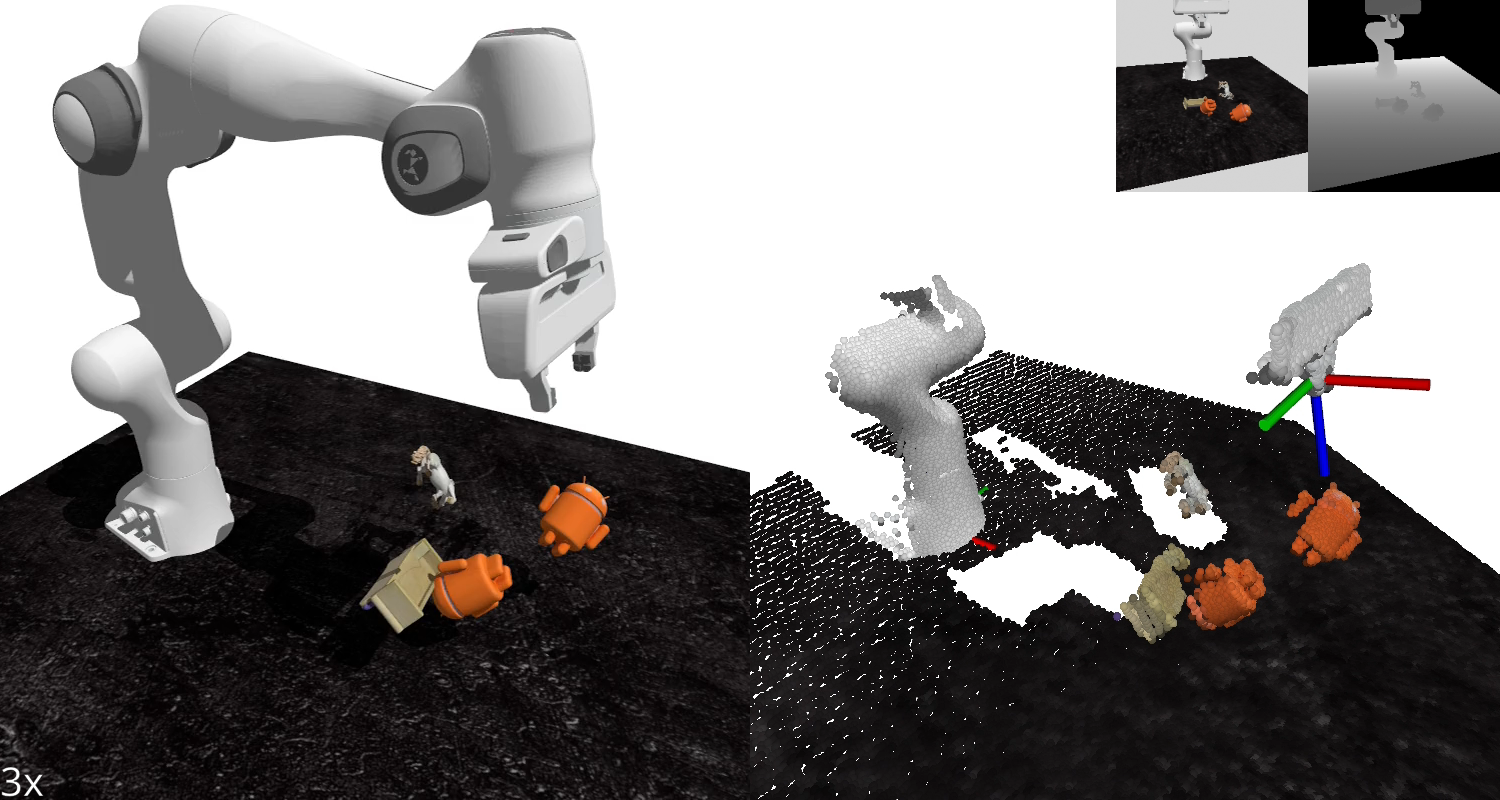
\includegraphics[width=\vidwidth,height=\vidheight]{videos/sim_panda_0.png}}{VPlayer.swf}
    }
\end{frame}

\begin{frame}{Results}{Invariance to Robot - Training and Evaluation}
    \begin{columns}%
        \begin{column}{0.55\textwidth}%
            \centering
            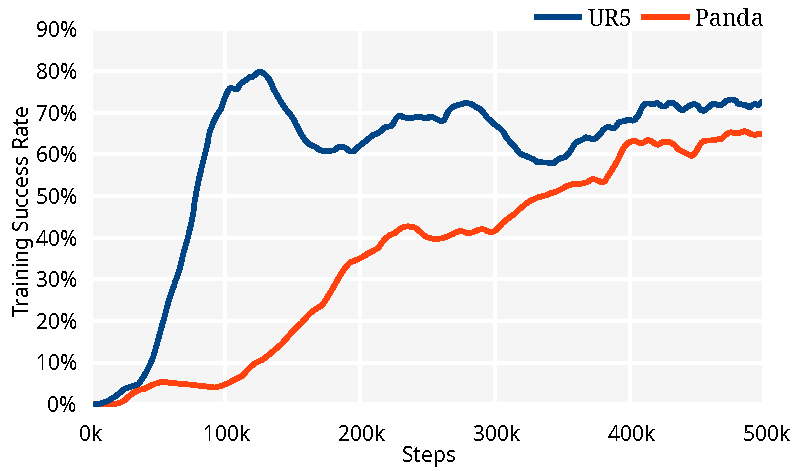
\includegraphics[height=4.25cm]{graphics/results_ue5_panda_robot.pdf}
        \end{column}
        %
        \begin{column}{0.45\textwidth}%
            \centering
            \begin{tabular}{c|cc}
                                               & \textbf{UR5} & \textbf{Panda} \\ \hline
                \begin{tabular}[c|]{@{}c@{}}Success\\Rate\end{tabular} & 77\%         & 61.5\%         \\[4mm]
                \begin{tabular}[c|]{@{}c@{}}Episode\\Length\end{tabular} & 14.0         & 27.1
            \end{tabular}
        \end{column}
    \end{columns}
\end{frame}

\begin{frame}{Results}{Sim-to-Real Transfer - Setup}
    \begin{columns}%
        \begin{column}{0.45\textwidth}%
            \centering
            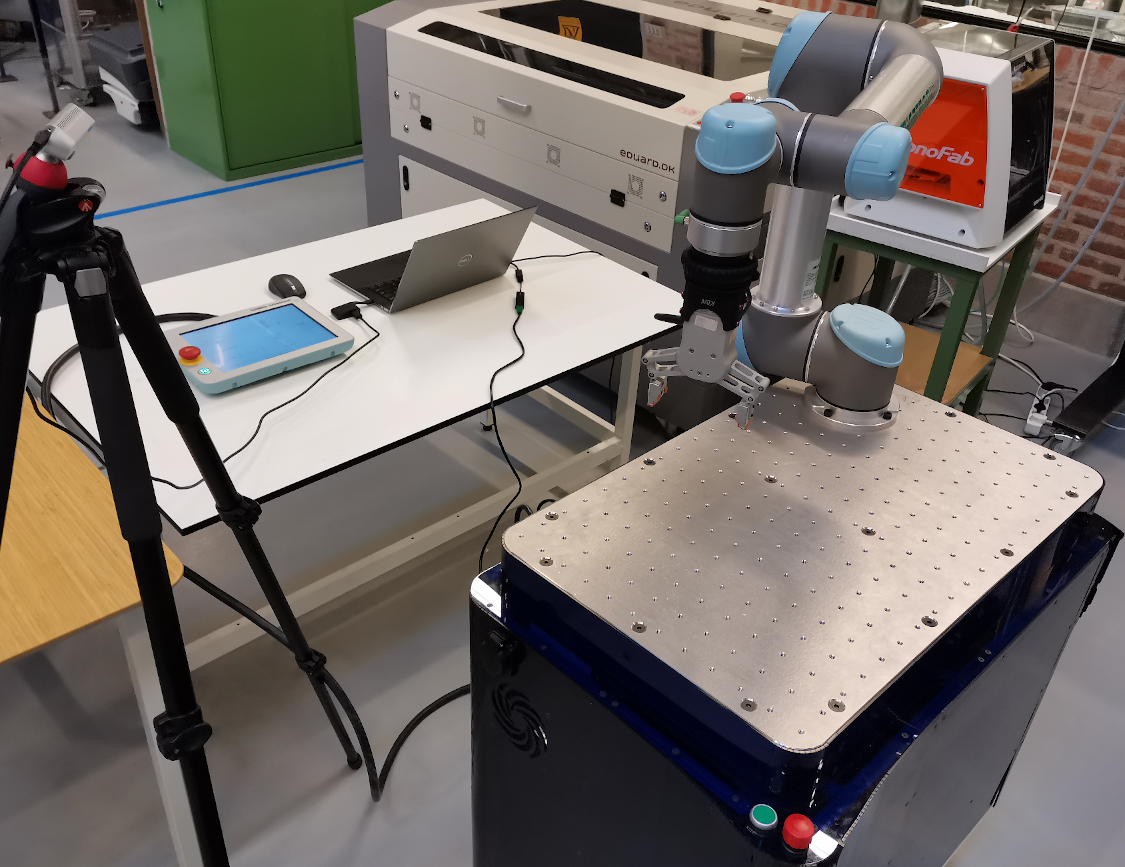
\includegraphics[width=\textwidth]{graphics/real_setup.png}
        \end{column}
        %
        \begin{column}{0.55\textwidth}%
            \centering
            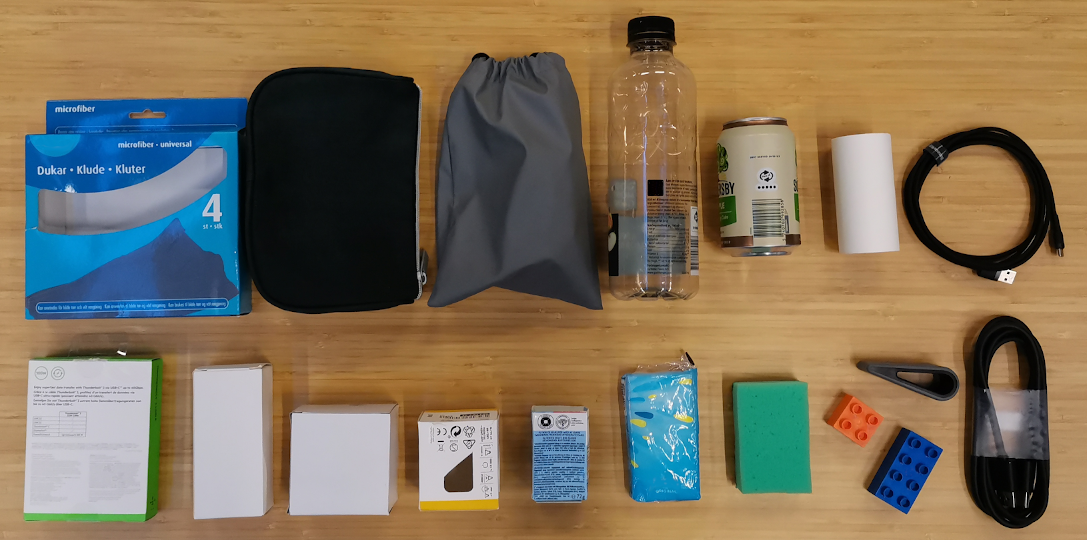
\includegraphics[width=\textwidth]{graphics/real_objects.png}
        \end{column}
    \end{columns}
\end{frame}

\begin{frame}{Results}{Sim-to-Real Transfer (Video Example)}
    \centering
    \scalebox{0.175}{%
        \def \vidwidth{2240px}%
        \def \vidheight{1000px}%
        \includemedia[width=\vidwidth,height=\vidheight,activate=pageopen,
            passcontext,
            transparent,
            keepaspectratio,
            final,
            noplaybutton,
            addresource=videos/sim2real.mp4,
            flashvars={source=videos/sim2real.mp4 &loop=true}
        ]{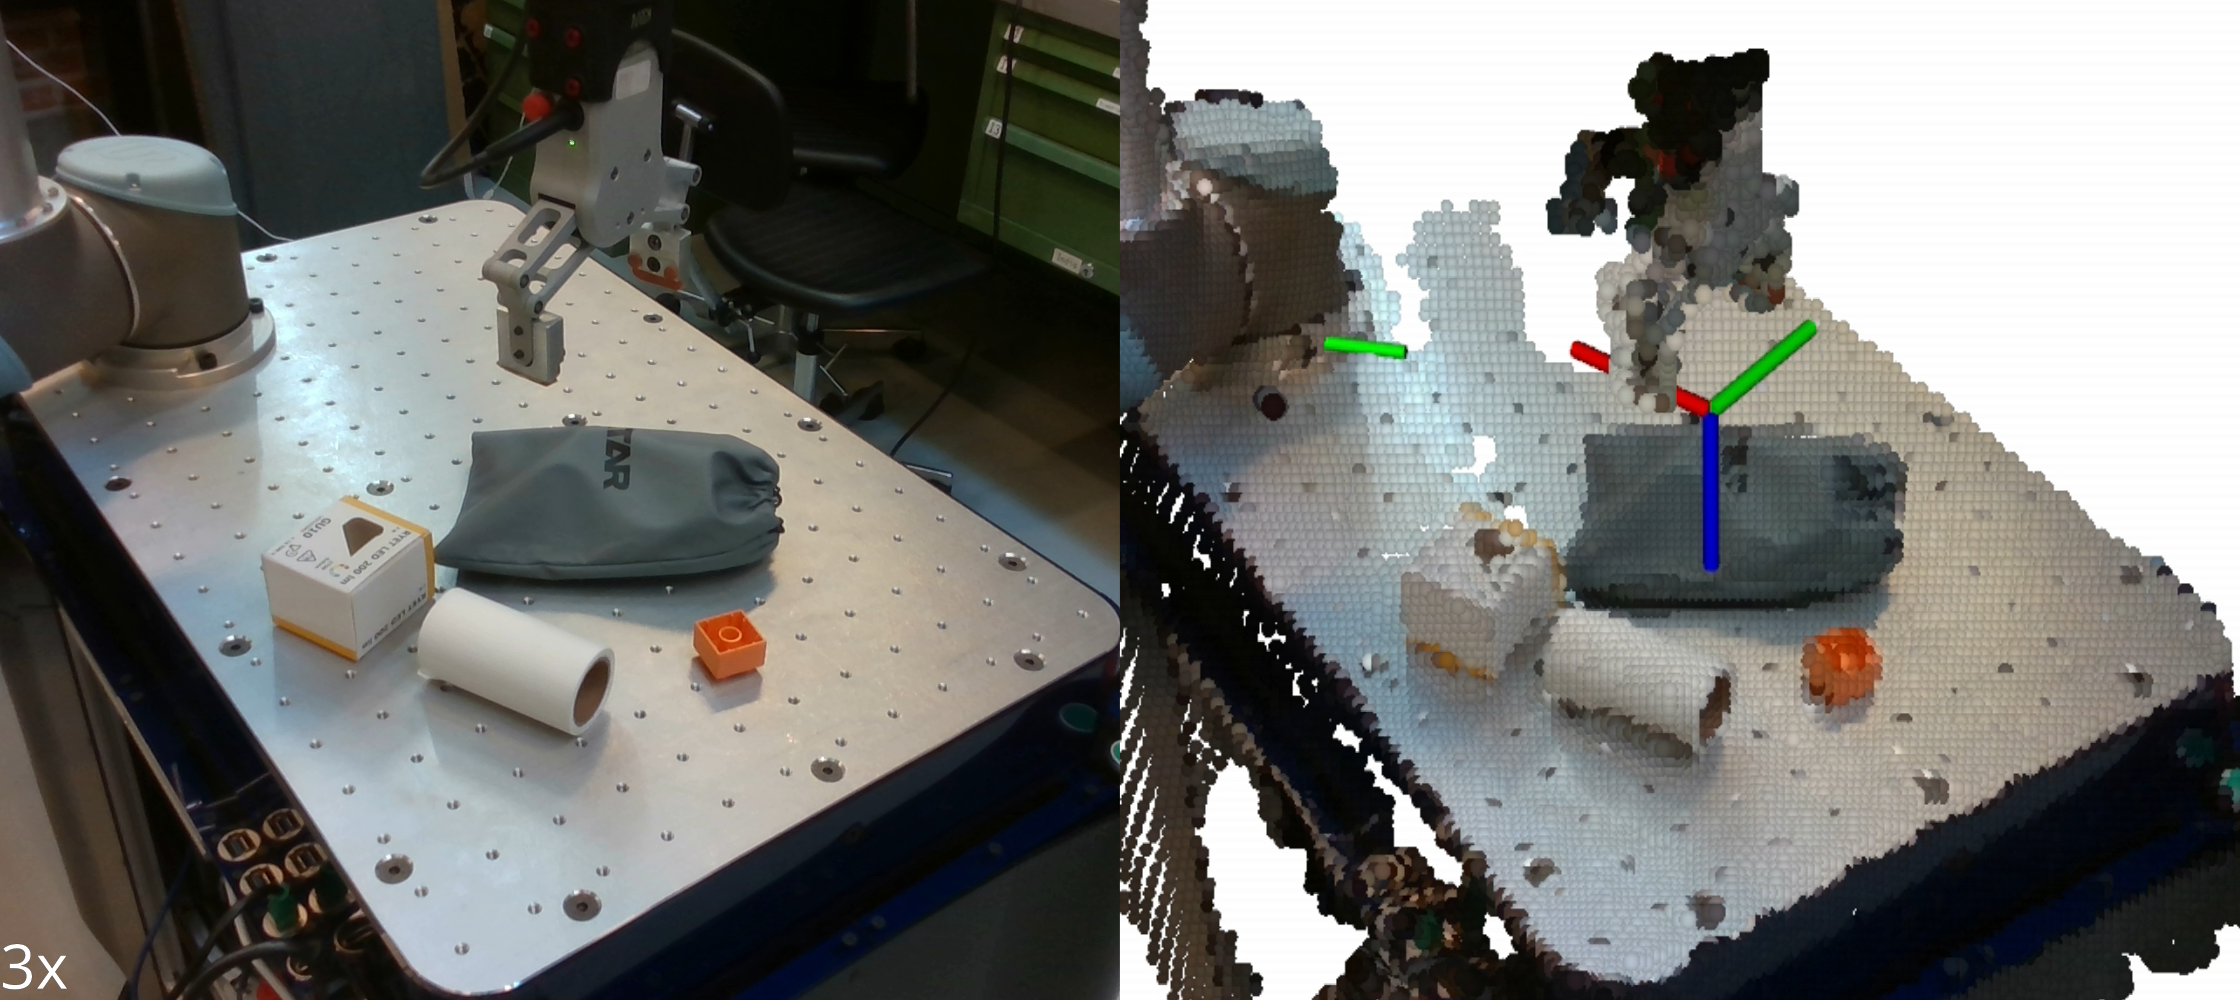
\includegraphics[width=\vidwidth,height=\vidheight]{videos/sim2real_0.png}}{VPlayer.swf}
    }
\end{frame}

% Add video with failures

\begin{frame}{Results}{Ablation Studies}
    \centering
    \vspace{-0.5cm}
    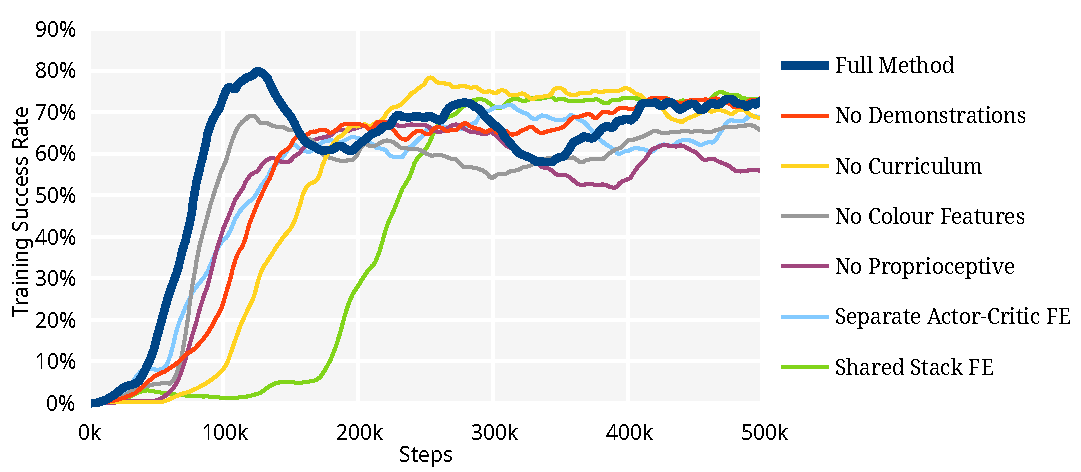
\includegraphics[height=4.5cm]{graphics/results_ablation_studies.pdf}

    \vspace{0.25cm}

    \resizebox{0.75\textwidth}{!}{%
        \begin{tabular}{c|ccccccc}
                                                    &
            \textbf{\begin{tabular}[c]{@{}c@{}}Full\\Method\end{tabular}} &
            \textbf{\begin{tabular}[c]{@{}c@{}}No\\Demon-\\strations\end{tabular}} &
            \textbf{\begin{tabular}[c]{@{}c@{}}No\\Curriculum\end{tabular}} &
            \textbf{\begin{tabular}[c]{@{}c@{}}No\\Colour\\Features\end{tabular}} &
            \textbf{\begin{tabular}[c]{@{}c@{}}No\\Proprio-\\ceptive\end{tabular}} &
            \textbf{\begin{tabular}[c]{@{}c@{}}Separate\\Actor-\\Critic FE\end{tabular}} &
            \textbf{\begin{tabular}[c]{@{}c@{}}Shared\\Stack\\FE\end{tabular}}                                                        \\ \hline
            \begin{tabular}[c|]{@{}c@{}}Success\\Rate\end{tabular}          & 77\% & 84\% & 70.5\% & 66.5\% & 75\% & 68.5\% & 79\% \\[4mm]

            \begin{tabular}[c|]{@{}c@{}}Episode\\Length\end{tabular}          & 14.0 & 24.5 & 19.9   & 29.4   & 23.0 & 27.5   & 22.8
        \end{tabular}}
\end{frame}


\section{Conclusion}

\begin{frame}[fragile]{Conclusion}{}
    \begin{block}{Primary Contributions}
        \begin{itemize}
            \item Simulation environment with domain randomisation
            \item Octree observations for end-to-end grasping with DRL
        \end{itemize}
    \end{block}

    \begin{block}{Performance and Scalability}
        \begin{itemize}
            \item Slow data collection and training
            \item Parallel workers are needed, with asynchronous updates of policy
        \end{itemize}
    \end{block}

    \begin{block}{Reproducibility}
        \begin{itemize}
            \item Not great for DRL
            \item Pre-built Docker image
        \end{itemize}
        \vspace{-0.2cm}
        \begin{lstlisting}[language=bash,basicstyle=\tiny,stepnumber=1,numbersep=10pt,tabsize=4,showspaces=false,showstringspaces=false]
        drl_grasping/docker/run.bash andrejorsula/drl_grasping:latest ros2 run drl_grasping ex_enjoy_pretrained_agent.bash
        \end{lstlisting}
    \end{block}
\end{frame}

\begin{frame}{Perspective on Reinforcement Learning}{}
    \centering
    \begin{block}{Great approach for learning complex robotics tasks! However, ...}\end{block}
    
    \vspace{0.2cm}
    
    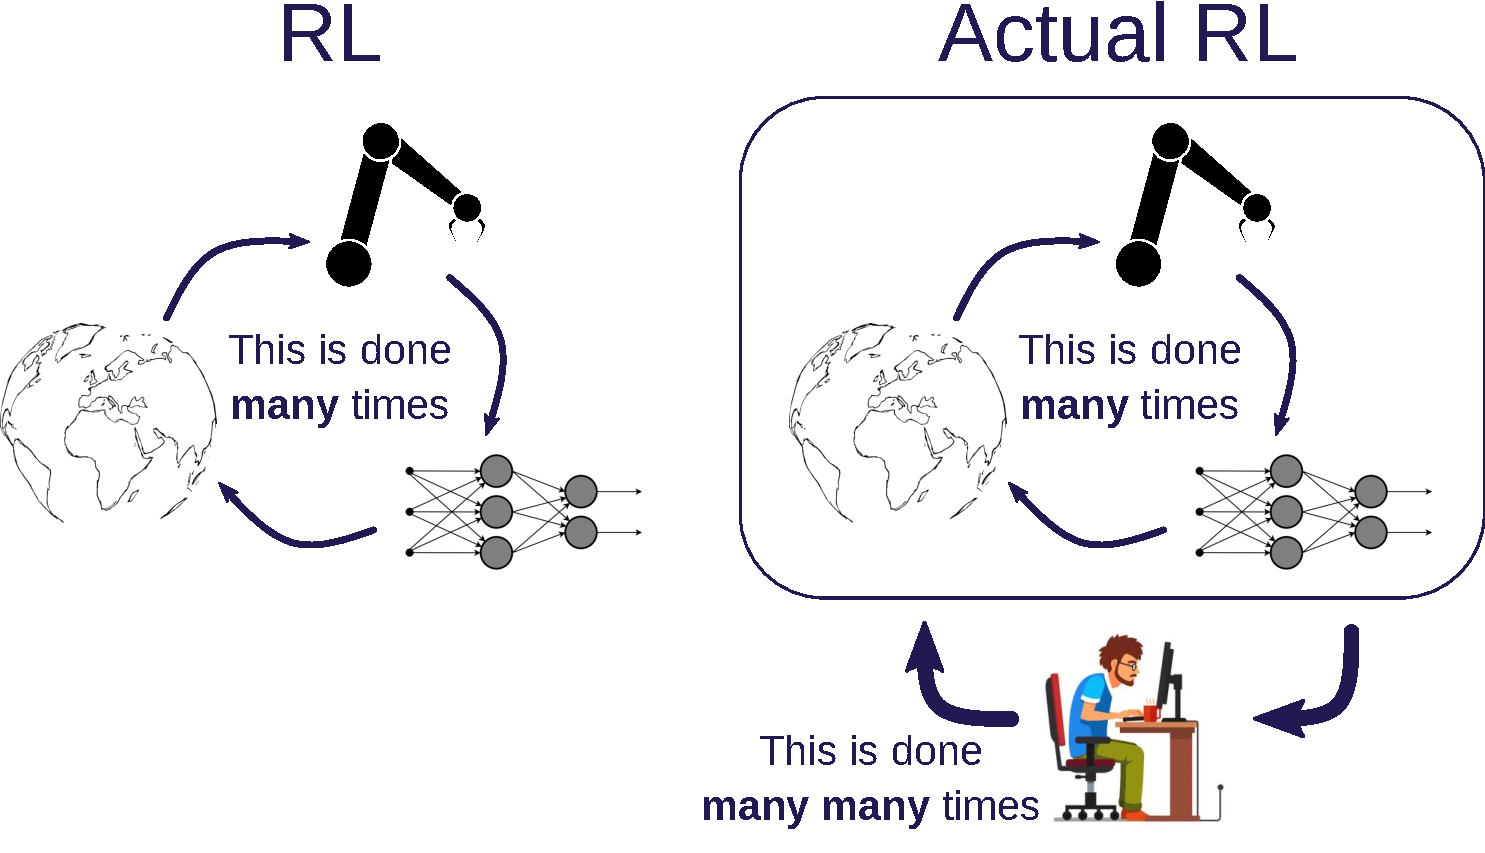
\includegraphics[height=5.2cm]{graphics/actual_rl.pdf}
    \footnoteref{Inspired by: Sergey Levine. 2020. CS 285 at UC Berkeley - L23}
\end{frame}
